\documentclass[12pt]{amsart}
\usepackage[utf8]{inputenc}
% Packages
\RequirePackage{amsmath,amssymb,amsthm}
\RequirePackage{amsfonts}
%\RequirePackage{geometry}
\RequirePackage{color}
\RequirePackage{mathtools}
\RequirePackage{bbm}
\RequirePackage{amsfonts}
\RequirePackage{mathrsfs}
\RequirePackage{tikz}
\usepackage[shortlabels]{enumitem}
\usetikzlibrary{shapes.geometric, arrows}
\usetikzlibrary{decorations.pathmorphing}
\usetikzlibrary{cd}
\tikzstyle{arrow} = [thick,->,>=stealth]

% Arrows
\providecommand{\po}{\arrow[ul,phantom,"\ulcorner" very near start]}
\providecommand{\pb}{\arrow[dr,phantom,"\lrcorner" very near start]}
\providecommand{\xto}[1]{\xrightarrow{#1}}
\providecommand{\from}{\leftarrow}
\providecommand{\xfrom}[1]{\overset{#1}{\leftarrow}}

\providecommand{\mapsfrom}{\mathrel{\reflectbox{\ensuremath{\mapsto}}}}
\providecommand{\longmapsfrom}{\mathrel{\reflectbox{\ensuremath{\longmapsto}}}}

\providecommand{\hookto}{\xhookrightarrow{}}
\providecommand{\xhookto}[1]{\overset{#1}{\hookrightarrow}}

\providecommand{\hookfrom}{\xhookleftarrow{}}
\providecommand{\xhookfrom}[1]{\xhookleftarrow{#1}}

\providecommand{\tto}{\twoheadrightarrow}
\providecommand{\xtto}[1]{\overset{#1}{\twoheadrightarrow}}
\providecommand{\ffrom}{\twoheadleftarrow}
\providecommand{\xffrom}[1]{\overset{#1}{\ffrom}}

\providecommand{\ladjoint}[2]{ #1\rightleftarrows #2 }
\makeatletter
\providecommand{\superimpose}[2]{%
  {\ooalign{$#1\@firstoftwo#2$\cr\hfil$#1\@secondoftwo#2$\hfil\cr}}}
\makeatother
\providecommand{\smallslash}{\mbox{\tiny/}}

\providecommand{\clhookto}{\mathrel{\raisebox{0.1em}{$\mathrel{\mathpalette\superimpose{{\hspace{0.1cm}\vspace{0.1em}\smallslash}{\hookrightarrow}}}$}}}
\providecommand{\xclhook}[1]{\overset{#1}{\clhook}}

\providecommand{\clhookfrom}{\mathrel{\raisebox{0.1em}{$\mathrel{\mathpalette\superimpose{{\hspace{0.1cm}\vspace{0.1em}\smallslash}{\hookleftarrow}}}$}}}

\providecommand{\ohookto}{\mathrel{\raisebox{0.03em}{$\mathrel{\mathpalette\superimpose{{\hspace{0.1cm}\vspace{0.03em}\mbox{\small$\circ$}}{\hookrightarrow}}}$}}}

\providecommand{\ohookfrom}{\mathrel{\raisebox{0.03em}{$\mathrel{\mathpalette\superimpose{{\hspace{0.1cm}\vspace{0.03em}\mbox{\small$\circ$}}{\hookleftarrow}}}$}}}

\providecommand{\cofto}{\rightarrowtail}
\providecommand{\coffrom}{\leftarrowtail}
\providecommand{\xcofto}[1]{\overset{#1}{\cofto}}
\providecommand{\xcoffrom}[1]{\overset{#1}{\coffrom}}

% Common Text Commands
\providecommand{\ab}{\text{ab}}
\providecommand{\ann}{\text{ann}}
\providecommand{\Aut}{\text{Aut}}
\providecommand{\char}{\text{char}}
\providecommand{\cl}{\text{cl}}
\providecommand{\codim}{\text{codim}}
\providecommand{\coev}{\text{coev}}
\providecommand{\colim}{\text{colim}}
\providecommand{\conj}{\text{conj}}
\providecommand{\const}{\text{const}}
\providecommand{\Disc}{\text{Disc}}
\providecommand{\End}{\text{End}}
\providecommand{\EKL}{\text{EKL}}
\providecommand{\ev}{\text{ev}}
\providecommand{\Fix}{\text{Fix}}
\providecommand{\Frac}{\text{Frac}}
\providecommand{\Frob}{\text{Frob}}
\providecommand{\Fun}{\text{Fun}}
\providecommand{\Gal}{\text{Gal}}
\providecommand{\GL}{\text{GL}}
\providecommand{\gr}{\text{gr}}
\newcommand{\GW}{\text{GW}}
\providecommand{\Hom}{\text{Hom}}
\providecommand{\id}{\text{id}}
\providecommand{\im}{\text{im}}
\renewcommand{\Im}{\text{Im}}
\providecommand{\incl}{\text{incl}}
\providecommand{\Ind}{\text{Ind}}
\providecommand{\Inn}{\text{Inn}}
\providecommand{\Jac}{\text{Jac}}
\providecommand{\Map}{\text{Map}}
\providecommand{\mult}{\text{mult}}
\providecommand{\op}{\text{op}}
\providecommand{\Orb}{\text{Orb}}
\providecommand{\ord}{\text{ord}}
\providecommand{\Out}{\text{Out}}
\providecommand{\Perm}{\text{Perm}}
\providecommand{\pr}{\text{pr}}
\providecommand{\pre}{\text{pre}}
\providecommand{\PSL}{\text{PSL}}
\providecommand{\quot}{\text{quot}}
\providecommand{\rank}{\text{rank}}
\renewcommand{\Re}{\text{Re}}
\providecommand{\Res}{\text{Res}}
\providecommand{\sgn}{\text{sgn}}
\providecommand{\sig}{\text{sig}}
\providecommand{\SL}{\text{SL}}
\providecommand{\soc}{\text{soc}}
\providecommand{\spn}{\text{span}}
\providecommand{\Spec}{\text{Spec}\hspace{0.1em}}
\providecommand{\Stab}{\text{Stab}}
\providecommand{\supp}{\text{supp}}
\providecommand{\Syl}{\text{Syl}}
\providecommand{\syl}{\text{syl}}
\providecommand{\Sym}{\text{Sym}}
\providecommand{\Tor}{\text{Tor}}
\providecommand{\Tr}{\text{Tr}}

% BB Sets
\providecommand{\A}{\mathbb{A}}
\providecommand{\C}{\mathbb{C}}
\providecommand{\F}{\mathbb{F}}
\providecommand{\N}{\mathbb{N}}
\providecommand{\P}{\mathbb{P}}
\providecommand{\Q}{\mathbb{Q}}
\providecommand{\R}{\mathbb{R}}
\providecommand{\Z}{\mathbb{Z}}

% Commands
\providecommand{\lrangle}[1]{\left\langle #1 \right\rangle}
\providecommand{\nsubgp}{\trianglelefteq}
\providecommand{\p}{\mathfrak{p}}
\renewcommand{\H}{\textbf{H}}
\newcommand{\gw}[1]{\left\langle #1 \right\rangle}
\newcommand{\ovl}[1]{\overline{#1}}

\let\minus\smallsetminus
\let\bar\overline
\let\smsh\wedge

\providecommand{\SH}{\mathcal{SH}}


% Colors
\providecommand{\green}[1]{\textcolor{green}{#1}}
\providecommand{\red}[1]{\textcolor{red}{#1}}
\providecommand{\orange}[1]{\textcolor{orange}{#1}}
\providecommand{\green}[1]{\textcolor{green}{#1}}
\providecommand{\blue}[1]{\textcolor{blue}{#1}}
\providecommand{\purple}[1]{\textcolor{purple}{#1}}

\RequirePackage{amsmath,amssymb}
\RequirePackage{geometry}

% AT commands
\providecommand{\BG}{\text{BG}}
\providecommand{\BO}{\text{BO}}
\providecommand{\BP}{\text{BP}}
\providecommand{\BU}{\text{BU}}
\providecommand{\BSO}{\text{BSO}}
\providecommand{\BSU}{\text{BSU}}
\providecommand{\BGL}{\text{BGL}}
\providecommand{\coeq}{\text{coeq}}
\providecommand{\cof}{\text{cof}}
\providecommand{\cone}{\text{cone}}
\providecommand{\eq}{\text{eq}}
\providecommand{\EU}{\text{EU}}
\providecommand{\Ex}{\text{Ex}}
\providecommand{\Ext}{\text{Ext}}
\providecommand{\Gr}{\text{Gr}}
\providecommand{\Ho}{\text{Ho}}
\providecommand{\hocofib}{\text{hocofib}}
\providecommand{\hocolim}{\text{hocolim}}
\providecommand{\holim}{\text{holim}}
\providecommand{\KGL}{\text{KGL}}
\providecommand{\ko}{\text{ko}}
\providecommand{\KO}{\text{KO}}
\providecommand{\kq}{\text{kq}}
\providecommand{\KQ}{\text{KQ}}
\providecommand{\KR}{\text{KR}}
\providecommand{\ku}{\text{ku}}
\providecommand{\KU}{\text{KU}}
\providecommand{\Lan}{\text{Lan}}
\providecommand{\MGL}{\text{MGL}}
\providecommand{\MO}{\text{MO}}
\providecommand{\MSL}{\text{MSL}}
\providecommand{\MSO}{\text{MSO}}
\providecommand{\MSp}{\text{MSp}}
\providecommand{\MU}{\text{MU}}
\providecommand{\Out}{\text{Out}}
\providecommand{\pre}{\text{pre}}
\providecommand{\Ran}{\text{Ran}}
\providecommand{\RO}{\text{RO}}
\providecommand{\Sing}{\text{Sing}}
\providecommand{\SO}{\text{SO}}
\providecommand{\Spin}{\text{Spin}}
\providecommand{\Sq}{\text{Sq}}
\providecommand{\SU}{\text{SU}}
\providecommand{\Sym}{\text{Sym}}
\providecommand{\TC}{\text{TC}}
\providecommand{\Th}{\text{Th}}
\providecommand{\THH}{\text{THH}}
\providecommand{\TP}{\text{TP}}
\providecommand{\TR}{\text{TR}}
\providecommand{\SH}{\mathcal{SH}}
\providecommand{\Sp}{\textit{Sp}}

% Chromatic
\providecommand{\Prin}{\text{Prin}}
\providecommand{\FGL}{\texttt{FGL}}
\providecommand{\SI}{\texttt{SI}}
\providecommand{\FG}{\text{FG}}
\providecommand{\fg}{\text{fg}}




% Spaces
\providecommand{\CP}{\mathbb{C}\text{P}}
\providecommand{\HP}{\mathbb{H}\text{P}}
\providecommand{\RP}{\mathbb{R}\text{P}}

% Other
\providecommand{\Cech}{\check{C}}
\let\adj\dashv
\let\smashprod\wedge


% Custom Arrows
% 
% (c) Thomas Brazelton
%
%% This program can be redistributed and/or modified under the terms
%% of the LaTeX Project Public License Distributed from CTAN archives
%% in directory macros/latex/base/lppl.txt.
% 

% Packages
\RequirePackage{amsmath,amssymb}
\RequirePackage{amsfonts}
\RequirePackage{geometry}
%\RequirePackage{hyperref}
\RequirePackage{color}
\RequirePackage{mathtools}		% used for arrows
%\RequirePackage{ bbold }
\RequirePackage{bbm}
\RequirePackage{amsfonts}
\RequirePackage{mathrsfs}
\RequirePackage{tikz}
%\usepackage[shortlabels]{enumitem}
\usetikzlibrary{shapes.geometric, arrows}
\usetikzlibrary{decorations.pathmorphing}
\usetikzlibrary{cd}
\tikzstyle{arrow} = [thick,->,>=stealth]


% Arrows
\providecommand{\po}{\arrow[ul,phantom,"\ulcorner" very near start]}
\providecommand{\pb}{\arrow[dr,phantom,"\lrcorner" very near start]}
\providecommand{\pol}{\arrow[ur,phantom,"\urcorner" very near start]}
\providecommand{\pbr}{\arrow[dl,phantom,"\llcorner" very near start]}
\providecommand{\xto}[1]{\xrightarrow{#1}}
\providecommand{\from}{\leftarrow}
\providecommand{\xfrom}[1]{\overset{#1}{\leftarrow}}

\providecommand{\mapsfrom}{\mathrel{\reflectbox{\ensuremath{\mapsto}}}}
\providecommand{\longmapsfrom}{\mathrel{\reflectbox{\ensuremath{\longmapsto}}}}

\providecommand{\hookto}{\xhookrightarrow{}}
\providecommand{\xhookto}[1]{\overset{#1}{\hookrightarrow}}

\providecommand{\hookfrom}{\xhookleftarrow{}}
\providecommand{\xhookfrom}[1]{\xhookleftarrow{#1}}

\providecommand{\tto}{\twoheadrightarrow}
\providecommand{\xtto}[1]{\overset{#1}{\twoheadrightarrow}}
\providecommand{\ffrom}{\twoheadleftarrow}
\providecommand{\xffrom}[1]{\overset{#1}{\ffrom}}

\providecommand{\ladjoint}[2]{ #1\rightleftarrows #2 }
\makeatletter
\providecommand{\superimpose}[2]{%
  {\ooalign{$#1\@firstoftwo#2$\cr\hfil$#1\@secondoftwo#2$\hfil\cr}}}
\makeatother
\providecommand{\smallslash}{\mbox{\tiny/}}

\providecommand{\clhookto}{\mathrel{\raisebox{0.1em}{$\mathrel{\mathpalette\superimpose{{\hspace{0.1cm}\vspace{0.1em}\smallslash}{\hookrightarrow}}}$}}}
\providecommand{\xclhook}[1]{\overset{#1}{\clhook}}

\providecommand{\clhookfrom}{\mathrel{\raisebox{0.1em}{$\mathrel{\mathpalette\superimpose{{\hspace{0.1cm}\vspace{0.1em}\smallslash}{\hookleftarrow}}}$}}}

\providecommand{\ohookto}{\mathrel{\raisebox{0.03em}{$\mathrel{\mathpalette\superimpose{{\hspace{0.1cm}\vspace{0.03em}\mbox{\small$\circ$}}{\hookrightarrow}}}$}}}

\providecommand{\ohookfrom}{\mathrel{\raisebox{0.03em}{$\mathrel{\mathpalette\superimpose{{\hspace{0.1cm}\vspace{0.03em}\mbox{\small$\circ$}}{\hookleftarrow}}}$}}}

\providecommand{\cofto}{\rightarrowtail}
\providecommand{\coffrom}{\leftarrowtail}
\providecommand{\xcofto}[1]{\overset{#1}{\cofto}}
\providecommand{\xcoffrom}[1]{\overset{#1}{\coffrom}}

\providecommand{\lllarrows}{\mathrel{\substack{\textstyle\leftarrow\\[-0.6ex] \textstyle\leftarrow \\[-0.6ex] \textstyle\leftarrow}}}



\providecommand{\rrrarrows}{\mathrel{\substack{\textstyle\rightarrow\\[-0.6ex] \textstyle\rightarrow \\[-0.6ex] \textstyle\rightarrow}}}

\providecommand{\rlrarrows}{\mathrel{\substack{\textstyle\rightarrow\\[-0.6ex] \textstyle\lefttarrow \\[-0.6ex] \textstyle\rightarrow}}}


\RequirePackage{cust-package-free}






% BB Sets
\providecommand{\C}{\mathbb{C}}
\providecommand{\F}{\mathbb{F}}
\providecommand{\N}{\mathbb{N}}
\providecommand{\Q}{\mathbb{Q}}
\providecommand{\R}{\mathbb{R}}
\providecommand{\Z}{\mathbb{Z}}

% Projective
\providecommand{\CP}{\mathbb{C}\text{P}}
\providecommand{\RP}{\mathbb{R}\text{P}}

% Colors
\providecommand{\green}[1]{\textcolor{green}{#1}}
\providecommand{\red}[1]{\textcolor{red}{#1}}
\providecommand{\orange}[1]{\textcolor{orange}{#1}}
\providecommand{\green}[1]{\textcolor{green}{#1}}
\providecommand{\blue}[1]{\textcolor{blue}{#1}}
\providecommand{\purple}[1]{\textcolor{purple}{#1}}

% Commands
\providecommand{\ceil}[1]{\left\lceil #1 \right\rceil}
\providecommand{\floor}[1]{\left\lfloor #1 \right\rfloor}
\providecommand{\lrangle}[1]{\left\langle #1 \right\rangle}
\providecommand{\und}[1]{\underline{#1}}
\renewcommand{\hat}{\widehat}
\providecommand{\legendre}[2]{\left( \substack{#1 \\ #2} \right)}
\providecommand{\trianglerightneq}{\mathrel{\ooalign{\raisebox{-0.5ex}{\reflectbox{\rotatebox{90}{$\nshortmid$}}}\cr$\triangleright$\cr}\mkern-3mu}}
\providecommand{\triangleleftneq}{\mathrel{\reflectbox{$\trianglerightneq$}}}

% Other
\providecommand{\dot}{\bullet}
\let\oldemptyset\emptyset
\let\emptyset\varnothing
\providecommand{\setminus}{\smallsetminus}
\providecommand{\minus}{\smallsetminus}
\let\bar\overline
\let\tilde\widetilde
\let\til\widetilde
\let\nsubgp\trianglelefteq
\let\del\partial
\let\epsilon\varepsilon
\providecommand{\bigast}{\mathop{\scalebox{1.5}{\raisebox{-0.2ex}{$\ast$}}}}
\providecommand{\llangle}{\left\langle\hspace{-0.2em}\left\langle}
\providecommand{\rrangle}{\right\rangle\hspace{-0.2em}\right\rangle}
\providecommand{\Pfister}[1]{\llangle #1 \rrangle}


% operp command for quadratic forms, from mathabx.sty
% https://tex.stackexchange.com/a/61882/
\DeclareFontFamily{U}{matha}{\hyphenchar\font45}
\DeclareFontShape{U}{matha}{m}{n}{
      <5> <6> <7> <8> <9> <10> gen * matha
      <10.95> matha10 <12> <14.4> <17.28> <20.74> <24.88> matha12
      }{}
\DeclareSymbolFont{matha}{U}{matha}{m}{n}
\DeclareFontFamily{U}{mathx}{\hyphenchar\font45}
\DeclareFontShape{U}{mathx}{m}{n}{
      <5> <6> <7> <8> <9> <10>
      <10.95> <12> <14.4> <17.28> <20.74> <24.88>
      mathx10
      }{}
\DeclareSymbolFont{mathx}{U}{mathx}{m}{n}
\DeclareMathSymbol{\operp}         {2}{matha}{"6B}
\DeclareMathSymbol{\bigoperp}       {1}{mathx}{"CB}



%%
%% End of file `custom-arrows.sty'.

\RequirePackage{amsmath,amssymb,amsfonts}
\RequirePackage{bbm}


% Categories
\providecommand{\onecat}{\mathbbm{1}}
\providecommand{\twocat}{\mathbbm{2}}
\providecommand{\Alg}{\texttt{Alg}}
\providecommand{\Ab}{\texttt{Ab}}
\providecommand{\CAlg}{\texttt{CAlg}}
\providecommand{\Cat}{\texttt{Cat}}
\providecommand{\CDGA}{\texttt{CDGA}}
\providecommand{\CG}{\texttt{CG}}
\providecommand{\CGWH}{\texttt{CGWH}}
\providecommand{\Ch}{\texttt{Ch}}
\providecommand{\CAlg}{\texttt{CAlg}}
\providecommand{\CMon}{\texttt{CMon}}
\providecommand{\coAlg}{\texttt{coAlg}}
\providecommand{\coMod}{\texttt{coMod}}
\providecommand{\Coh}{\texttt{Coh}}
\providecommand{\CommRing}{\texttt{CommRing}}
\providecommand{\Corr}{\texttt{Corr}}
\providecommand{\CRing}{\texttt{CRing}}
\providecommand{\CW}{\texttt{CW}}
\providecommand{\Field}{\texttt{Field}}
\providecommand{\Fin}{\texttt{Fin}}
\providecommand{\FinSet}{\texttt{FinSet}}
\providecommand{\Grp}{\texttt{Grp}}
\providecommand{\Grpd}{\texttt{Grpd}}
\providecommand{\Grph}{\texttt{Grph}}
\providecommand{\Kar}{\texttt{Kar}}
\providecommand{\Kan}{\texttt{Kan}}
\providecommand{\Mod}{\texttt{Mod}}
\providecommand{\lmod}[1]{#1\text{-}\texttt{Mod}}
\providecommand{\rmod}[1]{\texttt{Mod}\text{-}#1}
\providecommand{\bimod}[2]{#1\text{-}\texttt{Mod}\text{-}#2}
\providecommand{\Ouv}{\texttt{Ouv}}
\providecommand{\Poset}{\texttt{Poset}}
\providecommand{\PSh}{\texttt{PSh}}
\providecommand{\PShv}{\texttt{PShv}}
\providecommand{\qCat}{\texttt{qCat}}
\providecommand{\QCoh}{\texttt{QCoh}}
\providecommand{\Rep}{\texttt{Rep}}
\providecommand{\Ring}{\texttt{Ring}}
\providecommand{\Set}{\texttt{Set}}
\providecommand{\SH}{\mathcal{SH}}
\providecommand{\Sh}{\texttt{Sh}}
\providecommand{\Shv}{\texttt{Shv}}
\providecommand{\Spectra}{\texttt{Spectra}}
\providecommand{\sAb}{\text{sAb}}
\providecommand{\sSet}{\texttt{sSet}}
\providecommand{\Stack}{\texttt{Stack}}
\providecommand{\Top}{\texttt{Top}}
\providecommand{\Ring}{\texttt{Ring}}
\providecommand{\Vect}{\texttt{Vect}}

% Other
\providecommand{\cyc}{\text{cyc}}
\providecommand{\dg}{\text{dg}}
\providecommand{\gen}{\text{gen}}
\providecommand{\inj}{\text{inj}}
\providecommand{\mor}{\text{mor}}
\providecommand{\Mor}{\text{Mor}}
\providecommand{\ob}{\text{ob}}
\providecommand{\obj}{\text{obj}}
\providecommand{\proj}{\text{proj}}
\providecommand{\Span}{\text{Span}}

\newcommand{\DDelta}{\bm{\Delta}}


% Limits
\providecommand{\llim}{\varprojlim}
\providecommand{\rlim}{\varinjlim}




\usepackage{caption}
\usepackage{longtable}
\usepackage{quiver}
\usepackage{mdframed}
\usepackage{float}
\setlength{\parindent}{0em}
\setlength{\parskip}{0.5em}

\renewcommand{\P}{\mathbb{P}}
\let\til\widetilde



% Copied
\usepackage{xcolor}
\providecommand{\gray}[1]{\color{gray}#1 \color{black}}
\definecolor{purple}{RGB}{128, 0, 255} 
\renewcommand{\purple}[1]{\color{purple}#1 \color{black}}

\definecolor{darkgreen}{rgb}{0,0.30,0}
\renewcommand{\green}[1]{\color{darkgreen}#1 \color{black}}

\definecolor{darkred}{rgb}{0.75,0,0}
\newcommand{\darkred}[1]{\color{darkred}#1 \color{black}}

\definecolor{darkblue}{rgb}{0,0,0.6} 
\usepackage{amsthm,thmtools}
\usepackage[pdfborder=0,pagebackref,colorlinks,citecolor=darkgreen,linkcolor=darkgreen,urlcolor=darkblue]{hyperref}
\usepackage{cleveref}
    \let\fullref\autoref
%
%  \autoref is very crude.  It uses counters to distinguish environments
%  so that if say {lemma} uses the {theorem} counter, then autrorefs
%  which should come out Lemma X.Y in fact come out Theorem X.Y.  To
%  correct this give each its own counter eg:
%                 \newtheorem{theorem}{Theorem}[section]
%                 \newtheorem{lemma}{Lemma}[section]
%  and then equate the counters by commands like:
%                 \makeatletter
%                   \let\c@lemma\c@theorem
%                  \makeatother
%
%  To work correctly the environment name must have a corrresponding 
%  \XXXautorefname defined.  The following command does the job:
%
\def\makeautorefname#1#2{\expandafter\def\csname#1autorefname\endcsname{#2}}
%
%  Some standard autorefnames.  If the environment name for an autoref 
%  you need is not listed below, add a similar line to your TeX file:
%  
\makeautorefname{eqn}{Equation}%
\makeautorefname{sec}{Section}%
\makeautorefname{subsec}{Subsection}%
\makeautorefname{footnote}{footnote}%
\makeautorefname{item}{item}%
\makeautorefname{figure}{Figure}%
\makeautorefname{table}{Table}%
\makeautorefname{part}{Part}%
\makeautorefname{app}{Appendix}%
\makeautorefname{cla}{claim}%
\makeautorefname{conj}{conjecture}%
\makeautorefname{cor}{corollary}%
\makeautorefname{cex}{counterexample}%
\makeautorefname{cexs}{counterexamples}%
\makeautorefname{dig}{digression}%
\makeautorefname{disc}{discussion}%
\makeautorefname{def}{definition}%
\makeautorefname{ex}{example}%
\makeautorefname{exs}{examples}%
\makeautorefname{fac}{fact}%
\makeautorefname{intu}{intuition}%
\makeautorefname{lem}{lemma}%
\makeautorefname{meta}{metathm}%
\makeautorefname{nota}{notation}%
\makeautorefname{note}{note}%
\makeautorefname{prop}{proposition}%
\makeautorefname{rmk}{remark}%
\makeautorefname{term}{terminology}%
\makeautorefname{thm}{theorem}%
\makeautorefname{upsh}{upshot}%
%
%                  *** End of hyperref stuff ***



\theoremstyle{definition}
\newtheorem{theorem}{Theorem}[section]
\newtheorem{claim}[theorem]{Claim}
\newtheorem{conjecture}[theorem]{Conjecture}
\newtheorem{corollary}[theorem]{Corollary}
\newtheorem{counterexample}[theorem]{Counterexample}
\newtheorem{definition}[theorem]{Definition}
\newtheorem{digression}[theorem]{Digression}
\newtheorem{example}[theorem]{Example}
\newtheorem{examples}[theorem]{Examples}
\newtheorem{exercise}[theorem]{Exercise}
\newtheorem{fact}[theorem]{Fact}
\newtheorem{idea}[theorem]{Idea}
\newtheorem{intuition}[theorem]{Intuition}
\newtheorem{lemma}[theorem]{Lemma}
\newtheorem{metathm}[theorem]{Meta-theorem}

\newtheorem{notation}[theorem]{Notation}
\newtheorem{note}[theorem]{Note}
\newtheorem{proposition}[theorem]{Proposition}
\newtheorem{remark}[theorem]{Remark}
\newtheorem{terminology}[theorem]{Terminology}
\newtheorem{upshot}[theorem]{Upshot}



%\newtheorem{warning}[theorem]{Warning}

%%%% hack to get fullref working correctly
\makeatletter
\let\c@corollary=\c@theorem
\let\c@proposition=\c@theorem
\let\c@lemma=\c@theorem
\let\c@conjecture=\c@theorem
\let\c@definition=\c@theorem
\let\c@example=\c@theorem
\let\c@remark=\c@theorem
\let\c@notation=\c@theorem
\let\c@equation\c@theorem
\makeatother

\renewcommand*{\subsectionautorefname}{Subsection}
%%%%%%%%%%%%%%%%%%%%%%%%%%%%%%%%%%%%%%%%%%%%%%
\usepackage[color=lightblue,textsize=tiny]{todonotes}

\usepackage{fancyhdr}
\pagestyle{fancy}
\fancyhf{}
% \fancyhead[L]{\small\itshape\thespeaker}
% \fancyhead[R]{\small\itshape\theday, \theyear}
\fancyhead[C]{\small\itshape {\color{gray} Last compiled: \today}}
\fancyfoot[C]{\small {\thepage}}



\newcommand{\HZ}{H\widetilde{\mathbb{Z}}}

\providecommand{\GOS}{G\mathcal{O}\mathcal{S}}
\providecommand{\Pic}{\text{Pic}}
\providecommand{\Perf}{\text{Perf}}

\newcommand{\fiberq}[3]{\frac{#1}{#2}\hspace{-0.2em}{}_{#3}}

\renewcommand{\O}{\mathcal{O}}
\renewcommand{\Th}{\text{Th}}
\providecommand{\KO}{\text{KO}}

\let\del\partial
\providecommand{\soc}{\text{soc}}
\providecommand{\Sm}{\text{Sm}}
\providecommand{\ind}{\text{ind}}
\providecommand{\Vect}{\textit{Vect}}
\providecommand{\Char}{\text{char}}
\let\smashprod\wedge
\providecommand{\Sp}{\texttt{Sp}}
\providecommand{\TM}{\text{TM}}

\providecommand{\pt}{\text{pt}}

\providecommand{\Cof}{\text{Cof}}
\providecommand{\Fib}{\text{Fib}}
\providecommand{\LLP}{\text{LLP}}
\providecommand{\RLP}{\text{RLP}}
\let\emptyset\varnothing
\providecommand{\Cyl}{\text{Cyl}}

\title{Higher Algebra}

\author{Maximilien P\'eroux}
\date{\today}




\begin{document}

\maketitle

\begin{figure}[h]
  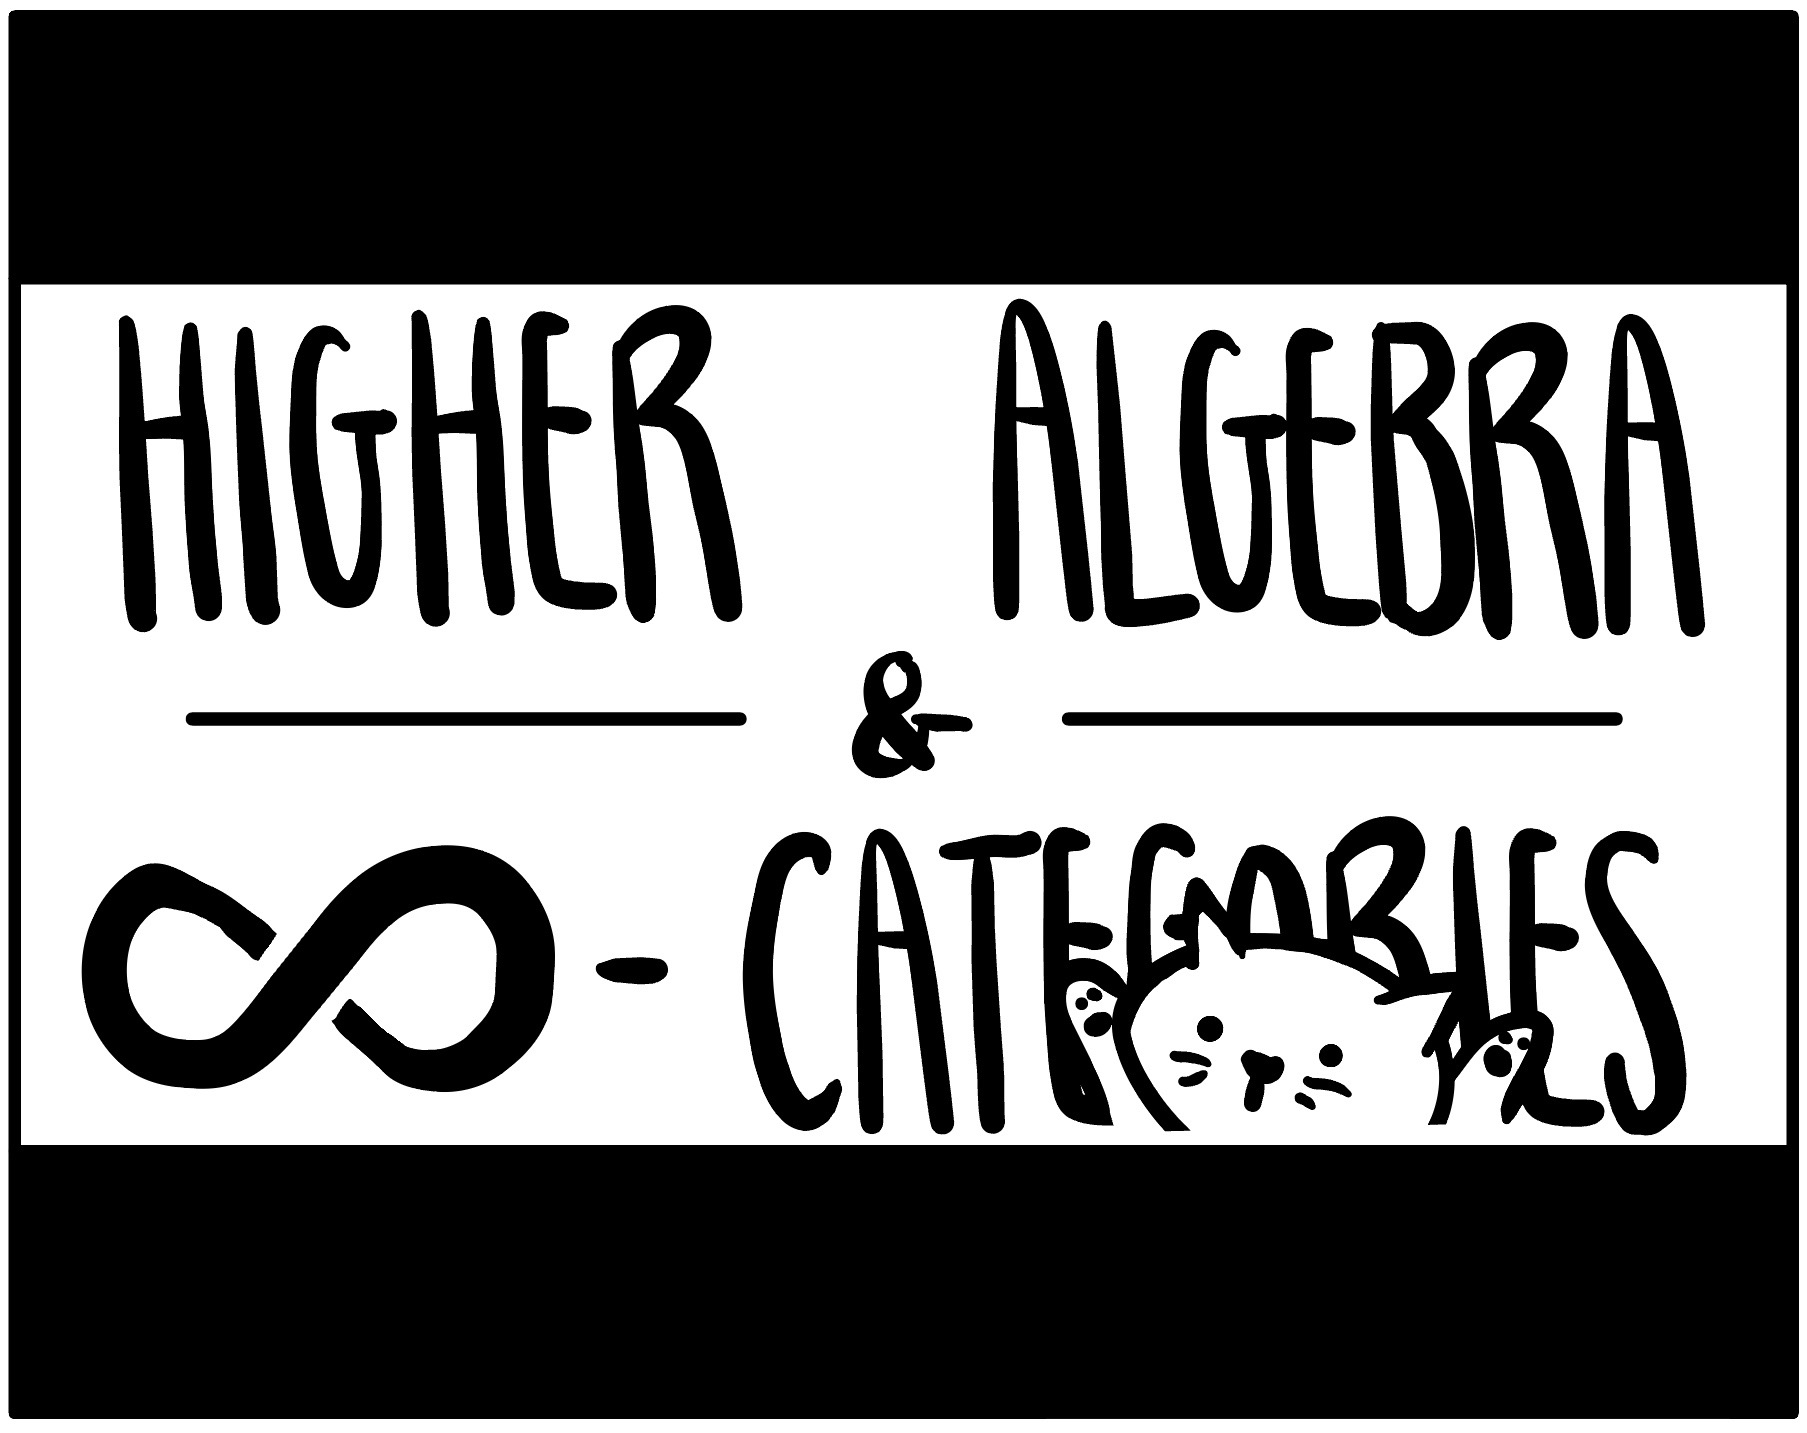
\includegraphics[width=0.5\linewidth]{pics/ha.jpg}
  \centering
  % \caption{}
  % \label{fig:}
\end{figure}


\section{Lecture 1: Thursday, January 12th}

Today: the \textbf{homotopy hypothesis}

\textbf{Classical algebra}: sets, monoids, groups, abelian groups, rings. Each of these are built up on the other. In higher courses, we may see groupoids, which are types of categories. A category is a generalization of a monoid, in some sense. We also have monoidal categories, which in some sense are a generalization of rings.

For higher algebra: spaces, $\mathbb{E}_1$-spaces, spectra, $\mathbf{E}_1$-ring spectra. Underlying this we have $\infty$-groupoids, $\infty$-categories, and monoidal $\infty$-categories.

We study spaces, not up to homeomorphism, but up to \textit{weak homotopy equivalence}. We will study this in a minute. ``Spaces'' in this class will always mean the study of topological spaces up to weak homotopy equivalence.

We'll give a synthetic definition of what an infinity category is, and circle back to a technical definition in about a month.

\textbf{What is an $\infty$-category}?

An $\infty$-category (or $(\infty,1)$-category) $\mathscr{C}$ should consist of:
\begin{enumerate}
    \item a class of objects
    \item a class of morphisms so that $\Hom_\mathscr{C}(X,Y)$ is a space
    \item $n$-morphisms for $n \ge 2$, where for instance 2-morphisms are between 1-morphisms, 3-morphisms between 2-morphisms, etc.
    \item morphisms can be composed in a suitable way
    \item $n$-morphisms for $n\ge 2$ are invertible in some sense.
\end{enumerate}

An $\infty$-groupoid (or $(\infty,0)$-category) should be an $\infty$-category where all the 1-morphisms are also invertible in some sense.

\textbf{Why study spaces up to weak homotopy equivalence}?

Recall by the Yoneda lemma, we have that
\begin{align*}
    X \cong Y \Leftrightarrow \Hom_\Top(A,X) \cong \Hom_\Top(A,Y)
\end{align*}
for all $A\in \Top$. Figuring out $\Hom(A,X)$ up to bijection for all $A$ is very difficult, so we prefer to study continuous maps up to homotopy. For $X$ and $Y$ nice enough, we say that $f\simeq g$ in $\Hom(X,Y)$ if there exists some path $I \to \Map(X,Y)$ so that $0 \mapsto f$ and $1 \mapsto g$. We define $[X,Y] = \Hom_\Top(X,Y)/\simeq$.

We see then that $X \simeq Y$ if and only if $[A,X] \cong [A,Y]$ for all $A \in \Top$.

We may ask when $[A,-] : \Top_\ast \to \Set$ factors through $\Grp$ or $\Ab$. We have that $[A,-]$ factors through $\Grp$ if and only if $A$ is a co-H-group in $\Top$. That is, we have maps
\begin{align*}
    A &\to A \vee A \\
    A &\to \ast,
\end{align*}
which is coassociative, counital, coinvertible.

\begin{example} $S^n$, when $n \ge 1$, is a co-H-space. The map $S^n \to S^n \vee S^n$ is the pinch map.
\end{example}

We say that $X$ is \textit{weakly homotopy equivalent} to $Y$, we write $X \sim Y$, if and only if there is a map $X \to Y$ inducing an isomorphism 
\[
\pi_n(X) = [S^n,X]_\ast \cong [S^n,Y]_\ast = \pi_n(Y),
\]
for all $n \ge 0$ (for $n \ge 1$ this is a group isomorphism).

If $X \sim Y$, then $H_n(X) \cong H_n(Y)$ for any $n$.

\begin{theorem} (Cellular approximation) For any $X$ in $\Top$, there exists $\til{X}$ a CW complex with a canonical map $\til{X} \xto{\sim} X$ that is a weak equivalence.
\end{theorem}

\begin{theorem} (Whitehead) If $X,Y$ are CW complexes, then $X \xto{\simeq} Y$ is a homotopy equivalence if and only if $X \xto{\sim} Y$ is a weak homotopy equivalence.
\end{theorem}

\begin{exercise} Find spaces $X$ and $Y$ which are weakly homotopy equivalent but not homotopy equivalent.
\end{exercise}

We denote by $\Delta$ the simplex category. Its objects are ordered sets of the form $[n] = \left\{ 0,1, \ldots, n \right\}$, and its morphisms are order-preserving maps. We have that $\Delta$ is generated by \textit{cofaces} and \textit{codegeneracies}. The cofaces are of the form
\begin{align*}
    d^0,d^1: [0] \to [1],
\end{align*}
skipping $0$ or $1$ in $[1]$, etc. The codegeneracies look like $s^0 : [1] \to [0]$ which ``repeat'' an element.

The cofaces and codegeneracies satisfy certain \textit{cosimplicial identities}.

If $\mathscr{C}$ is a category, we denote by $s \mathscr{C} = \mathscr{C}^{\Delta^\op}$ the simplicial objects in $\mathscr{C}$. If $\mathscr{C} = \Set$, we write $\sSet$ as the category of simplicial sets. A simplicial set $X_\bullet \in \sSet$ consists of sets $X_0, X_1, \ldots$ together with face and degeneracy maps satisfying the simplicial identities.

\begin{example} The \textit{nerve of a small category}. Let $\mathscr{C} \in \Cat$ a small category. We denote by $N_\bullet \mathscr{C}$ the simplicial set with $N_0 \mathscr{C} = \ob \mathscr{C}$, $N_1 \mathscr{C} = \mor \mathscr{C}$, and $N_n \mathscr{C}$ the set of $n$ composable morphisms in $\mathscr{C}$. That is,
\begin{align*}
    N_n \mathscr{C} = N_1 \mathscr{C} \times_{N_0 \mathscr{C}} \cdots \times_{N_0 \mathscr{C}} N_1 \mathscr{C}.
\end{align*}
The face maps are source/target/composition. The degeneracies insert an identity morphism.
\end{example}

\begin{example} Via Yoneda, we get a functor
\begin{align*}
    \Delta^n := \Hom_\Delta(-,[n]) : \Delta^\op \to \Set.
\end{align*}
If $X_\bullet$ is a simplicial set, we get that the set of $n$-simplices $X_n$ is in bijection with $\Hom_\sSet(\Delta^n, X_\bullet)$.
\end{example}

\begin{example} (Dold--Kan) We have $\Ch_R^{\ge 0} \xto{\Gamma} s\Mod_R$ is an isomorphism, where $\Gamma_m C_\bullet  =\oplus_{[n] \tto [k]} C_k$, with faces and degeneracies left as an exercise.
\end{example}

\begin{example} Let $\Delta^n_\Top \subseteq \R^{n+1}$ be defined by
\begin{align*}
    \left\{ (t_0, \ldots, t_n) \in \R^{n+1} \colon 0 \le t_i \le 1,\ \sum t_i = 1 \right\}.
\end{align*}
We can view $[n] = \left\{ v_0, \ldots, v_n \right\}$, and $v_i = (0, \ldots, 0,1,0, \ldots, 0)$ with 1 at the $i$th place. Then if $\alpha : [m] \to [n]$ in $\Delta$, we can define $\alpha(v_i) =v_{\alpha(i)}$. Extend linearly to get $\alpha_\ast : \Delta^m_\Top \to \Delta^n_\Top$. We get then that $\Delta^\bullet_\Top$ is a cosimplicial topological space.
\end{example}

\begin{example} If $X \in \Top$, we have $\Sing_\bullet(X) \in \sSet$ defined by $\Sing_n(X) = \Hom_\Top \left( \Delta_\Top^n, X \right)$.
\end{example}

\begin{definition} If $X_\bullet \in \sSet$, we define its \textit{geometric realization} to be
\begin{align*}
    |X_\bullet| = \amalg_{n\ge 0} X_n \times \Delta^n_\Top / \sim,
\end{align*}
where $(x,s)\sim (y,t)$ if and only if there is some $\alpha : [m] \to [n]$ so that $\alpha^\ast y = x$ and $\alpha_\ast s = t$.
\end{definition}


\begin{example} $|\Delta^n_\bullet| \cong \Delta^n_\Top$.
\end{example}

\begin{exercise} $|X_\bullet|$ is always a CW complex for any $X_\bullet \in \sSet$.
\end{exercise}

\begin{exercise} We have an adjunction $|-| : \sSet \leftrightarrows \Top: \Sing(-)$
\end{exercise}

\begin{definition} $X_\bullet \to Y_\bullet$ is a \textit{weak homotopy equivalence} in $\sSet$ if $|X_\bullet| \xto{\sim} |Y_\bullet|$ is a weak homotopy equivalence of spaces.
\end{definition}

\begin{theorem} (Quillen) Simplicial sets up to weak equivalence is equivalent to topological spaces up to weak homotopy equivalence. Moreover, for any $X\in \Top$, we have that $|\Sing(X)|$ is weakly equivalent to $X$.
\end{theorem}

\begin{figure}[h]
  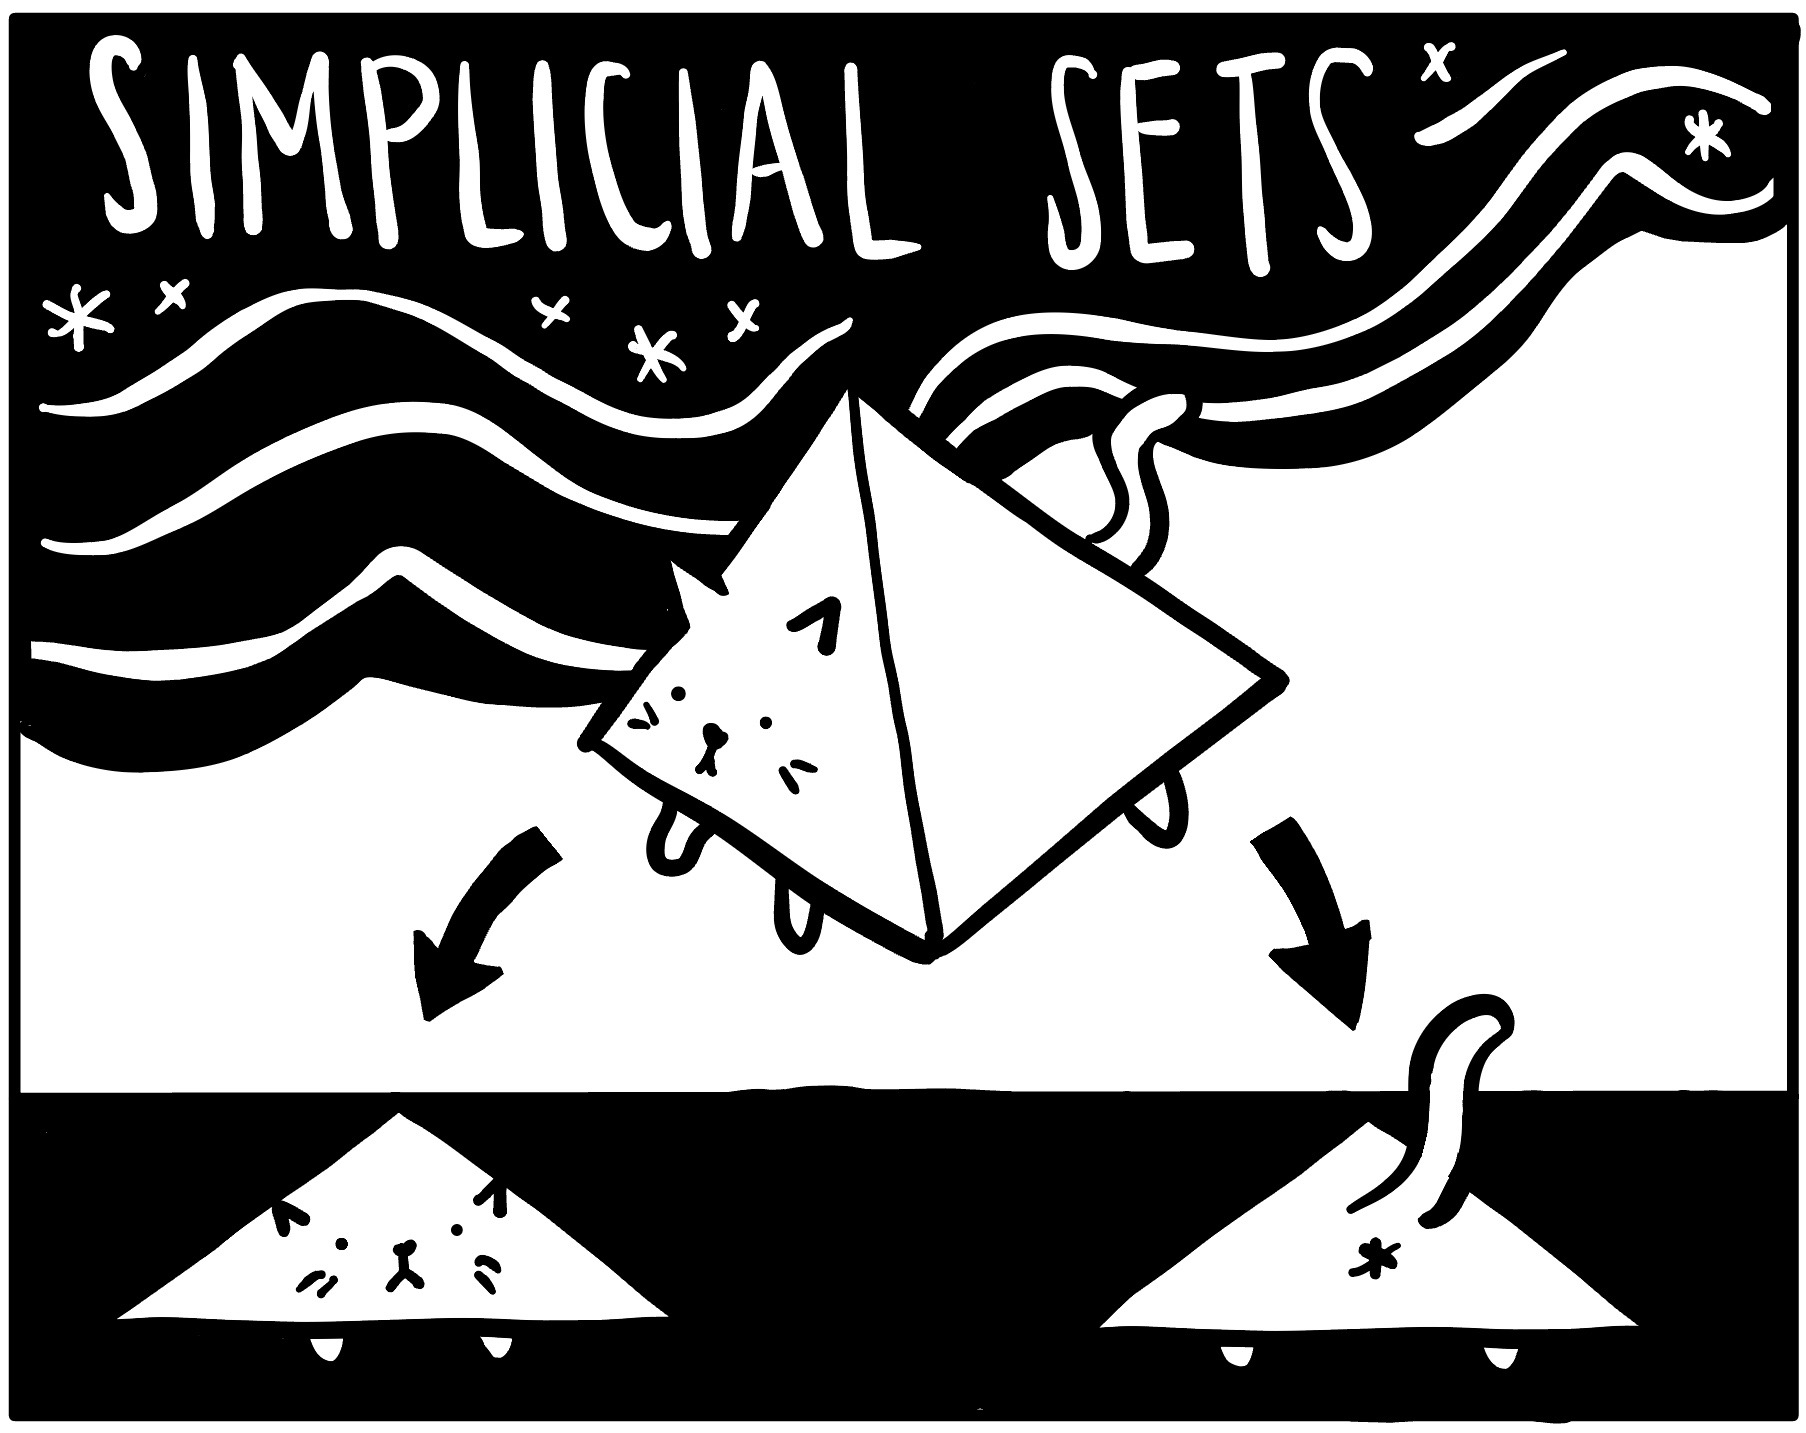
\includegraphics[width=0.5\linewidth]{pics/sset.jpg}
  \centering
 \end{figure}



\section{Lecture 2: Tuesday, January 17th}

\textbf{Today}: the homotopy hypothesis (continued).

Recall we are interested in studying $\Top$ up to weak homotopy equivalences. Equivalently, we are interested in studying $\sSet$ up to weak equivalence, and the relationship between the two was given by the geometric realization / singular complex adjunction.

Recall we've defined $\Delta^n = \Hom_\Delta(-,[n])$. We will define the $k$\textit{th horn} $\Lambda^n_k \subseteq \Delta^n$ as a coequalizer in $\sSet$
\begin{align*}
    \left(\coprod_{0 \le i < j \le n} \Delta^{n-2} \rightrightarrows \coprod_{i\ne k} \Delta^{n-1} \right) \to \Lambda^n_k,
\end{align*}
where the two maps are $\delta^{j-1}$ and $\delta^i$. The geometric realization of $\Lambda^n_k$ is the topological $n$-simplex, with the middle and the face opposite the $k$th edge removed.

\begin{definition} We say that $Y\in \sSet$ is a \textit{Kan complex} if for all $k\le n$, and for every $\Lambda^n_k \to Y$, there exists a (not necessarily unique) lift:
\[ \begin{tikzcd}
    \Lambda^n_k\dar[hook]\rar & Y\\
    \Delta^n\ar[ur,dashed] & 
\end{tikzcd} \]
\end{definition}

\begin{exercise} $Y$ is a Kan complex if and only if for any $(n-1)$-simplices $y_1, \ldots, y_{k-1},y_{k+1}, \ldots, y_n$ such that $d_i y_j = d_{j-1} y_i$ for $i< j$, $i,j\ne k$, there exists an $n$-simplex $y$ such that $d_i y = y_i$ for all $i\ne k$.
\end{exercise}

\begin{exercise} We have that $\Sing(X)$ is always a Kan complex for any $X\in \Top$.
\end{exercise}

\begin{exercise} We have that $\Delta^n$ is not a Kan complex for $n \ge 1$.
\end{exercise}

\begin{exercise} If $X \in s\Grp$, then the underlying simplicial set of $X$ is always a Kan complex.
\end{exercise}

Up to weak homotopy equivalence, every simplicial set is a Kan complex (will see this later).

Recall the Dold-Kan correspondence
\begin{align*}
    s\Mod_\Z \cong \Ch_\Z^{\ge 0},
\end{align*}
which sends weak homotopy equivalences to quasi-isomorphisms. Given a simplicial set $X_\ast$, we can take an associated simplicial abelian group $\Z[X_\ast]$ by taking the free group on $n$-simplices at level $n$. We can ask what $\Z[X_\ast]$ corresponds to as a chain complex. One answer is that
\begin{align*}
    \Z[\Sing(X_\ast)] \leftrightarrow C_\ast(X;\Z).
\end{align*}
This tells us that
\begin{align*}
    \pi_\ast \left( \Z \left[ \Sing(X) \right] \right) \cong H_\ast(X;\Z).
\end{align*}
In some sense we can view $\Z[\Sing(X)]$ as being (equivalent to) the \textit{free commutative monoid} on $X$. This is what is known as the \textit{Dold-Thom theorem}.

\textbf{Homotopy hypothesis}: Spaces (up to weak equivalence) are $\infty$-groupoids. For us, spaces up to weak equivalences correspond to Kan complexes.

Given $X\in \Kan$, we can call $X_0$ the objects, and $X_1$ the morphisms. The horn filling conditions on horns tell you that you can \textit{compose} and \textit{invert} morphisms in $X_1$, witnessed by simplices in $X_2$.

\begin{definition} A \textit{quasi-category} (i.e. $\infty$-category) is a simplicial set with inner horn lifting property. That is, we can lift against horns $\Lambda^n_k$ for $0<k<n$.
\end{definition}

\begin{exercise} A quasi-category has unique horn filling if and only if it is isomorphic to the nerve of a 1-category.
\end{exercise}

\begin{center}
\textbf{Model categories}
\end{center}

\textbf{Vista}: Every nice infinity category is equivalent in some sense to a model category. This will pretty much be the goal of this class.

\begin{notation} Let $\mathcal{M}$ be a category, and $\chi \subseteq \mathcal{M}$ a class of morphisms. We define $\LLP(\chi)$ to be the class of morphisms in $\mathcal{M}$ so that $f$ has left lifting property with respect to all morphisms in $\chi$:
\[\begin{tikzcd}
    \cdot\rar\dar["f" left] & \cdot\dar["\in\ \chi" right]\\
    \cdot\rar\ar[ur,dashed] & \cdot
\end{tikzcd} \]
\end{notation}

Similarly we can define $f\in \RLP(\chi)$ by
\[\begin{tikzcd}
    \cdot\rar\dar["\chi\ \ni" left] & \cdot\dar["f" right]\\
    \cdot\rar\ar[ur,dashed] & \cdot
\end{tikzcd} \]

\begin{figure}[h]
  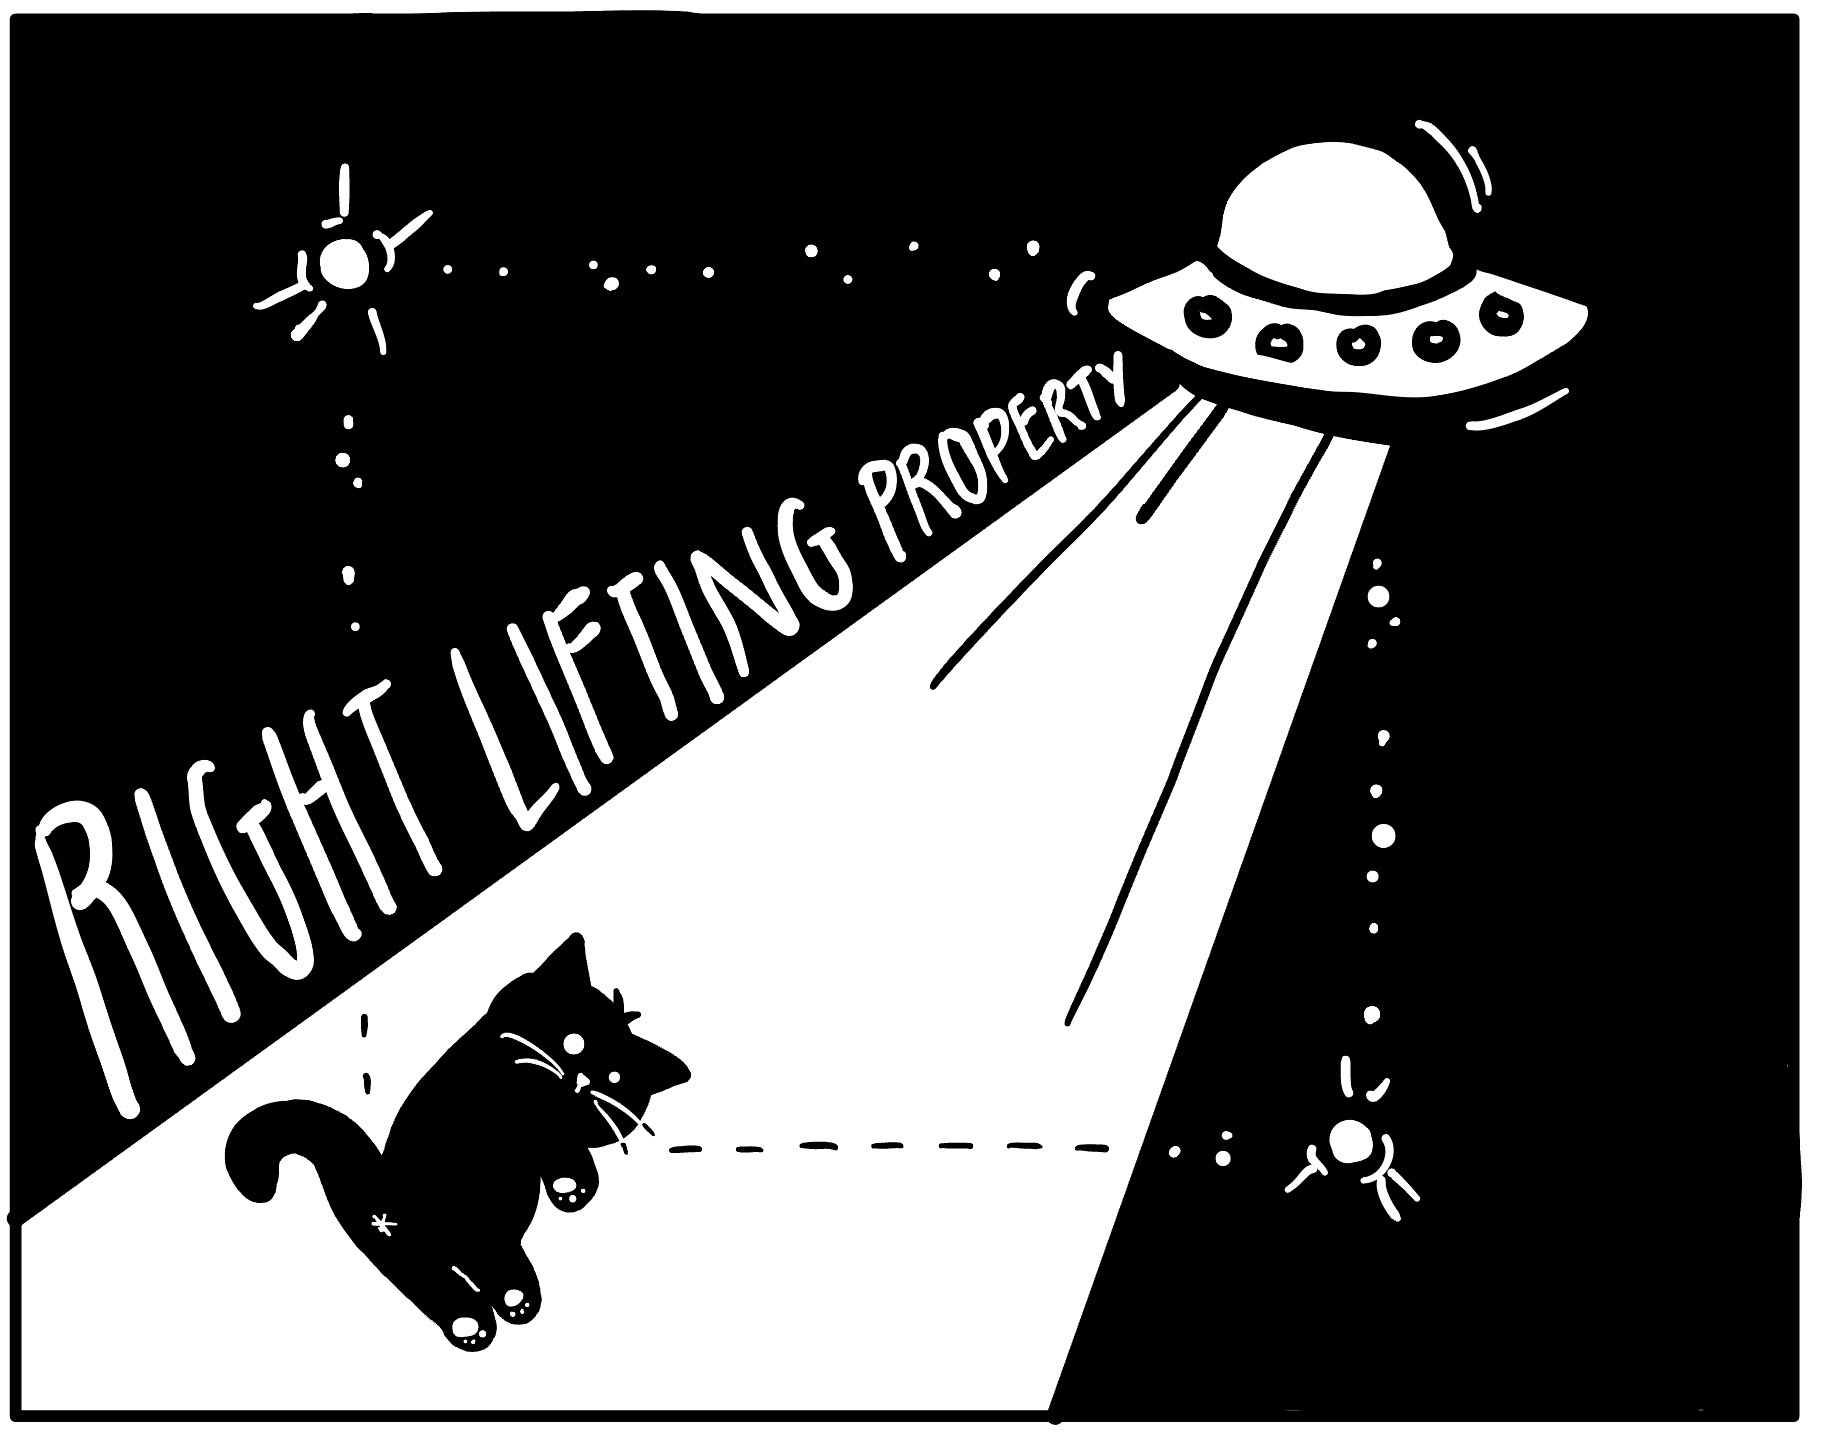
\includegraphics[width=0.5\linewidth]{pics/rlp.jpg}
  \centering
\end{figure}


\begin{definition} A \textit{weak factorization system} on a category $\mathcal{M}$ consists of a pair $(\mathscr{C}, \mathscr{F})$ of classes of morphisms such that
\begin{enumerate}
    \item Given any $f: X \to Y$ in $\mathcal{M}$, it factors (not necessarily uniquely) as
\[ \begin{tikzcd}
    X\ar[rr,"f" above]\ar[dr,"\mathscr{C}\ni" below left] &  & Y\\
     & W\ar[ur,"\in \mathscr{F}" below right] &
\end{tikzcd} \]

    \item $\mathscr{C} = \LLP(\mathscr{F})$ and $\mathscr{F} = \RLP(\mathscr{C})$.
\end{enumerate}
\end{definition}

\begin{example} In $\Set$, we have that mono and epimorphisms give a weak factorization system. A factorization is
\[ \begin{tikzcd}
    X\ar[rr,"f" above]\ar[dr,"\id_X \times f" below left] &  & Y\\
     & X \times Y\ar[ur,"\pi_Y" below right] & 
\end{tikzcd} \]
% The lifting property
% \[ \begin{tikzcd}
%     A\rar\dar[hook] & X\dar[two heads]\\
%     B\rar\ar[ur,dashed] & Y
% \end{tikzcd} \]
\end{example}

\begin{definition} A \textit{model structure} on $\mathcal{M}$ consists of three classes of morphisms:
\begin{center}
    \begin{tabular}{l | l}
    $W$ & weak equivalences \\
    $\Cof$ & cofibrations \\
    $\Fib$ & fibrations
    \end{tabular}
\end{center}
We denote by $\widetilde{\Cof}:= \Cof \cap W$ and $\widetilde{\Fib} = \Fib \cap W$, and call these \textit{trivial cofibrations} (resp. \textit{trivial fibrations}). These are subject to the constraint that
\begin{enumerate}
    \item $\mathcal{M}$ is bicomplete (all limits and colimits)\footnote{We might also require \textit{finitely} bicomplete.}
    \item $W$ satisfies 2-out-of-3 property\footnote{If $f$ and $g$ are composable, and any two of $f$, $g$, $gf$ are in $W$ then so is the third.}
    \item $\left( \Cof, \til{\Fib} \right)$ and $\left( \widetilde{\Cof}, \Fib \right)$ are weak factorization systems.
\end{enumerate}
\end{definition}

\begin{terminology} A category with a model structure is referred to as a \textit{model category}.
\end{terminology}

\begin{figure}[h]
  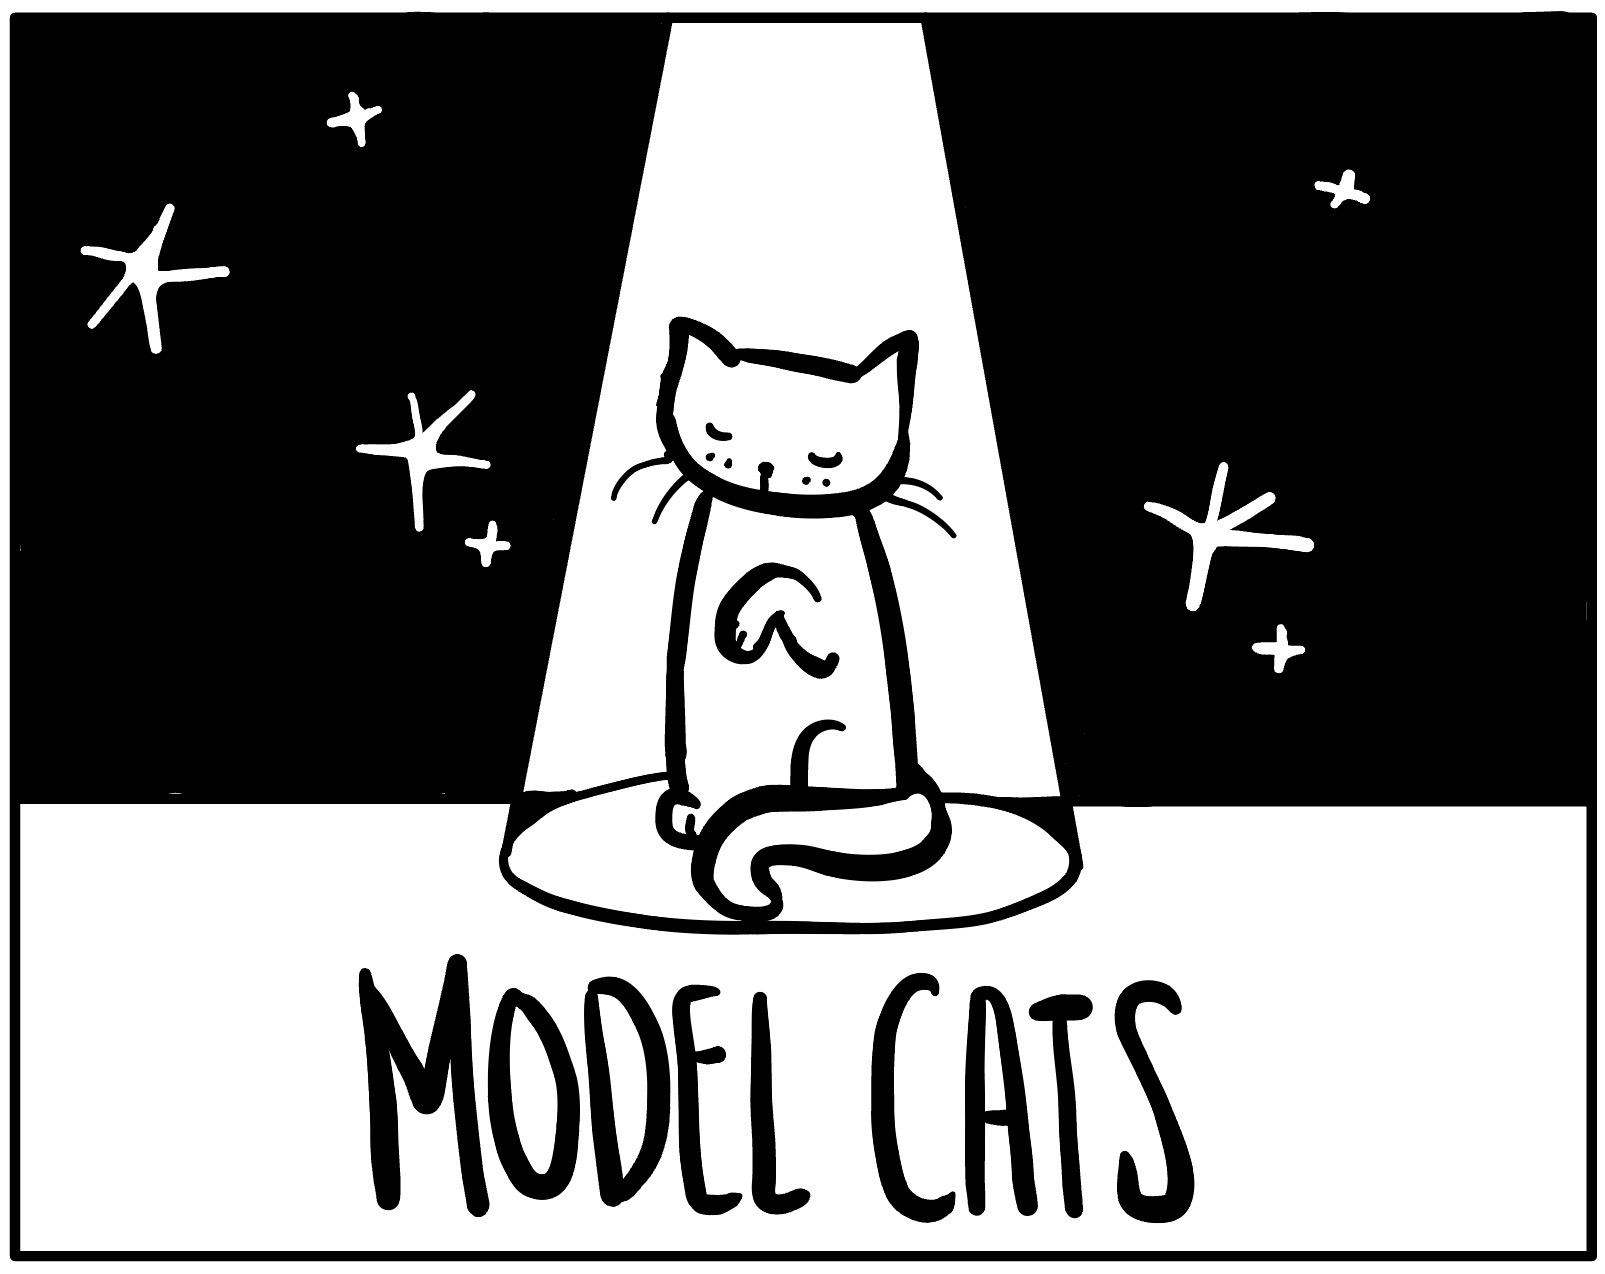
\includegraphics[width=0.5\linewidth]{pics/model-cats.jpg}
  \centering

\end{figure}


\begin{notation} We will decorate each class of morphisms as
\begin{center}
\begin{tabular}{l | l}
    $W$ & $\xto{\sim}$ \\
    $\Cof$ & $\hookto$ \\
    $\Fib$ & $\tto$
    \end{tabular}
\end{center}
\end{notation}


\begin{exercise} $W$, $\Cof$, and $\Fib$ are closed under retracts: that is,
\[ \begin{tikzcd}
    \cdot\dar["f" left]\rar\ar[rr,equal,bend left=20] & \cdot\dar["g"]\rar & \cdot\dar["f"]\\
    \cdot\rar\ar[rr,equal,bend right=20] & \cdot\rar & \cdot\\
\end{tikzcd} \]
then if $g\in W$ (resp. $\Cof$ or $\Fib$) then $f\in W$ (resp. $\Cof$ or $\Fib$).
\end{exercise}

\begin{definition} Let $\mathcal{M}$ be a model category, and let $\emptyset \in \mathcal{M}$ the initial object and $\ast\in \mathcal{M}$ the terminal object. 

\begin{itemize}
    \item We say that $X\in \mathcal{M}$ is \textit{cofibrant} if the unique map $\emptyset \to X$ is a cofibration. 
    \item We say that $X\in \mathcal{M}$ is \textit{fibrant} if the unique map $X \to \ast$ is a fibration.
    \item We say that $\til{X}$ is a \textit{cofibrant replacement} of $X$ if
\[ \begin{tikzcd}
    \emptyset\ar[rr]\ar[dr,hook] &  & X\\
     & \til{X}\ar[ur,two heads,"\sim" below right] & 
\end{tikzcd} \]
    \item We say that $\til{X}$ is a \textit{fibrant replacement} of $X$ if
\[ \begin{tikzcd}
    X\ar[rr]\ar[dr,hook,"\sim" below left] &  & \ast\\
     & \til{X}\ar[ur,two heads] & 
\end{tikzcd} \]
\end{itemize}
\end{definition}

\begin{example} $\mathcal{M} = \Top$, $W=$ weak homotopy equivalences, $\Cof=$ relative CW complexes\footnote{$A\hookto X$ is a \textit{relative CW complex} if $X$ is built out of $A$ by attaching cells.} The fibrations are determined by $\Fib = \RLP(\widetilde{\Cof})$. The fibrations are equivalently $\RLP(D^n \to D^n \times I)$. Every object here is fibrant, and the cofibrant objects are precisely the CW complexes. Cofibrant replacement is cellular approximation.
\end{example}

\section{Lecture 3: Thursday, January 19th}

\begin{proposition}\label{prop:labelname} Identities and isomorphisms are weak equivalences in a model category.
\end{proposition}
\begin{proof} For any $X \in \mathcal{M}$, we can fibrantly replace it to get $X \xhookto{\sim} \til{X}$. Consider the commutative diagram
\[ \begin{tikzcd}
    X\ar[rr,"\id"]\ar[dr,hook,"\sim" below left] &  & X\ar[dl,"\sim" below right]\\
     & \til{X}. & 
\end{tikzcd} \]
By 2-out-of-3, we have that $\id:X \to X$ is also a weak equivalence.

More generally if $f:X \to Y$ is an isomorphism in $\mathcal{M}$, then by the diagram
\[ \begin{tikzcd}
    X\dar["f" left]\rar["f" above]\ar[rr,equal,bend left=20] & Y\dar[equal]\rar["f^{-1}"] & X\dar["f" right]\\
    Y\rar[equal] & Y\rar[equal] & Y,
\end{tikzcd} \]
we see that $f$ is contained in $W$.
\end{proof}

If $\left( \mathscr{C},\mathscr{F} \right)$ is a weak factorization system, then both $\mathscr{C}$ and $\mathscr{F}$ are closed under retracts. Hence $\Cof, \til{\Cof}, \Fib, \til{\Fib}$ are closed under retracts. $W$ is also closed under retracts (exercise).

\begin{exercise} We have that $\mathcal{M}$ is a model category if and only if $\mathcal{M}^\op$ is a model category.
\end{exercise}

\begin{theorem} Cofibrations are closed under pushouts and coproducts.
\end{theorem}
\begin{proof} Given any test square, we can try to lift:
\[\begin{tikzcd}
    X\rar\dar[hook] & Y\rar\dar & A\dar[two heads,"\sim" right]\\
    Z\rar\ar[urr,dashed] & P\rar\po & B.
\end{tikzcd} \]
This map is constructed by universal property of the pushout:
\[ \begin{tikzcd}
    X\rar\dar[hook] & Y\dar\ar[ddr,bend left=10] & \\
    Z\rar\ar[drr,bend right=10,dashed] & P\po\ar[dr,dashed,"\exists!" above right] & \\
     &  & A.
\end{tikzcd} \]
For coproducts, we can take $X_i \hookto Y_i$ for $i\in J$. Let's try to lift:
\[ \begin{tikzcd}
    X_i\dar[hook]\rar & \amalg_i X_i\dar\rar & A\dar[two heads,"\sim" right]\\
    Y_i\rar\ar[urr,dashed] & \amalg_i Y_i\rar & B.
\end{tikzcd} \]
We know that each $X_i\hookto Y_i$ is a cofibration hence it lifts against the big square. By universal property a map $\amalg_i Y_i \to A$ exists.
\end{proof}


\begin{example} If $\mathscr{C}$ is a bicomplete category, then $\mathscr{C}$ has a model structure where $W$ is the isomorphisms, and $\Cof = \Fib = \mor \mathscr{C}$.
\end{example}

\begin{example} If $\mathcal{M} = \Top$, we have the \textit{Quillen model structure}, with
\begin{itemize}
    \item $W=$ weak homotopy equivalences
    \item $\Cof=$ retracts of relative CW complexes
    \item $\Fib=$ Serre fibrations ($\RLP(D^n \hookto D^n \times I)$).
\end{itemize}
\end{example}


\begin{example} The Str{\o}m (or Hurewicz) model structure on $\Top$:
\begin{itemize}
    \item $W=$ homotopy equivalences
    \item $\Fib=$ Hurewicz fibrations ($\RLP(A \to A \times I)$ for all $A \in \Top$)
    \item $\Cof=$ closed cofibrations in $\Top$.
\end{itemize}
Fibrant replacement in the Str{\o}m model structure looks like
\[ \begin{tikzcd}
    X\ar[rr,"f"]\ar[dr,hook] &  & Y\\
     & M_f\ar[ur,two heads,"\simeq" below right] &
\end{tikzcd} \]
Where $M_f = (X \times I)\cup_X Y$ is the mapping cylinder.
\end{example}

\begin{example} The \textit{Kan model structure} on $\sSet$ with
\begin{itemize}
    \item $W=$ weak homotopy equivalences
    \item $\Cof=$ monomorphisms (levelwise injections)
    \item $\Fib=$ Kan fibrations ($\RLP(\Lambda_k^n \to \Delta^n)$ for all $0\le k\le n$).
\end{itemize}
Everything is cofibrant here (since the empty simplicial set injects into everything). Fibrant things are Kan complexes. This tells us that every simplicial set is weakly equivalent to a Kan complex!
\end{example}

\begin{theorem} (Milnor) The natural map $X \to \Sing(|X|)$ is a weak homotopy equivalence for any simplicial set $X$. [Kerodon, 3.5.4.1]
\end{theorem}


\begin{definition} Let $\mathscr{C}$ be a cat, and $W \subseteq \mathscr{C}$ a subcategory. A functor $F: \mathscr{C} \to \mathscr{D}$ is called the \textit{localization of $\mathscr{C}$ with respect to $W$} if:
\begin{enumerate}
    \item $F(f) \in \text{iso} \mathscr{D}$ if $f\in \mor W$
    \item For any other $F'$ satisfying (1), we have
\[ \begin{tikzcd}
    \mathscr{C}\rar["F'"]\dar["F" left] & \mathscr{D}'\\
    \mathscr{C}\ar[ur,"\exists!" below right] & 
\end{tikzcd} \]
\end{enumerate}
We denote by $\mathscr{C} \to \mathscr{C}[W^{-1}]$ the localization.
\end{definition}

Here is a naive way to construct $\mathscr{C}[W^{-1}]$: we take the free category on $\mathscr{C}$ and ``$W^{-1}$.'' That is, we take the same objects, but allow morphisms to be ``zigzags'' of morphisms forward in $\mathscr{C}$ and morphisms backwards in $W$, and we mod out by the relation that things in $W$ become isomorphisms. There are size issues here.

\begin{theorem} If $\mathcal{M}$ is a model category, then localization $\mathcal{M} \to \mathcal{M}[W^{-1}]$ exists. We denote by $\Ho(\mathcal{M}) = \mathcal{M}[W^{-1}]$ the homotopy category of $\mathcal{M}$.
\end{theorem}

Recall in $\Top$ that $f \simeq g : X \to Y$ if there is a map $H: X \times I \to Y$ so that $H(-,0) = f$ and $H(-,1) = g$. 

\begin{definition} Le t$\mathcal{M}$ be a model category. A \textit{cylinder object} on $X\in \mathcal{M}$ is defined to be
\[ \begin{tikzcd}
    X\amalg X\ar[rr,"\nabla"]\ar[dr,hook] &  & Y\\
     & \Cyl(X)\ar[ur,"\sim" below right] &
\end{tikzcd} \]
The construction of cylinder objects is \textit{not functorial}.
\end{definition}

A \textit{(left) homotopy} from $f$ to $g$ is a map $H: \Cyl(X) \to Y$ such that $H\circ i_0 = f$ and $H\circ i_1 = g$. We denote this by $f\simeq g$.

\begin{proposition} We have that $i_0 : X \to \Cyl(X)$ is a weak equivalence (and same for $i_1$).
\end{proposition}
\begin{proof} We have
\[\begin{tikzcd}
    X\ar[rr,"\id", bend left=30]\ar[dr,dashed,"i_0" below left]\rar & X\amalg X\rar["\nabla"]\dar & Y\\
     & \Cyl(X)\ar[ur,"\sim" below right] & \\
\end{tikzcd} \]
By 2-out-of-3 on the outside maps, the result follows.
\end{proof}

\begin{proposition} If $X$ is cofibrant, then $i_0,i_1: X \to \Cyl(X)$ are cofibrations.
\end{proposition}
\begin{proof} Since cofibrations are preserved under pushouts, we have that $i_0$ and $i_1$ are cofibrations:
\[ \begin{tikzcd}
    \emptyset\rar[hook]\dar[hook] & X\dar["i_0" right]\\
    X\rar["i_1" below] & X \amalg X \po
\end{tikzcd} \]
\end{proof}

\begin{theorem} (Exercise) If $X$ is cofibrant, then homotopy $\simeq$ gives an equivalence relation on $\Hom(X,Y)$ for any $Y$.
\end{theorem}

We can think of a map
\begin{align*}
    \Hom_\mathcal{M}(X,Y)/\simeq \times \Hom_\mathcal{M}(Y,Z)/\simeq &\to \Hom_\mathcal{M}(X,Z)/\simeq \\
    (f,g) &\mapsto g\circ f.
\end{align*}
In order for this to be well-defined, we need $Z$ to be fibrant.

\begin{lemma} If $Z$ is fibrant, and $f\simeq g: X \to Z$, then if $h: X' \to X$, we have that $fh\simeq gh$.
\end{lemma}
\begin{proof} We have $H: \Cyl(X) \to Y$ with $H_0 = f$ and $H_1 = g$. By lifting, we get
\[ \begin{tikzcd}
    X'\amalg X'\rar\dar[hook] & X\amalg X\rar & \Cyl(X)\dar[two heads,"\sim" right]\\
    \Cyl(X')\rar\ar[urr,dashed] & X'\rar & X.
\end{tikzcd} \]
This gives the desired map. We used fibrancy of $Z$ to ensure that the map $\Cyl(X) \to X$ was a trivial fibration (or could be replaced with a better cylinder object using a map to $Z$).
\end{proof}

\begin{theorem} In $\mathcal{M}$, given $f: X \to Y$ with $X$ cofibrant and $Y$ fibrant, then $f\in W$ if and only if $f$ is a homotopy equivalence.\footnote{Meaning that there is some $g: Y \to X$ with $fg\simeq \id$ and $gf\simeq \id$.}
\end{theorem}

\begin{notation} $\mathcal{M}_c=$ cofibrant objects in $\mathcal{M}$, and $\mathcal{M}_f=$ fibrant objects in $\mathcal{M}$. We denote by $\mathcal{M}_{cf}=$ objects which are \textit{both} cofibrant and fibrant.
\end{notation}

Concretely, we can define $\Ho(\mathcal{M})$ as the objects in $\mathcal{M}$, but where
\begin{align*}
    \Hom_{\Ho(\mathcal{M})}(X,Y) = \Hom_{\mathcal{M}_{cf}/\simeq}(RQX,RQY),
\end{align*}
where $R$ is a fibrant replacement and $Q$ is a cofibrant replacement.

\begin{exercise} Given $X \to Y$ in $\mathcal{M}$, there exists $QX \xto{\til{f}} QY$ such that
\[ \begin{tikzcd}
    QX\dar[two heads,"\sim"]\rar["\til{f}"] & QY\dar[two heads,"\sim"]\\
    X\rar["f" below] & Y.
\end{tikzcd} \]
Here $\til{f}$ is well-defined up to left homotopy.
\end{exercise}

Given some $\mathcal{M} \to \Ho(\mathcal{M})$, we just need to check that $W \mapsto$ isos, and it is universal in that way.

\section{Lecture 4: Tuesday, January 24th}

\begin{definition} Suppose $\mathcal{M}$ and $\mathcal{N}$ are model categories, and take a functor $F: \mathcal{M} \to \mathcal{N}$. A \textit{left derived functor} of $F$ is an (absolute) right Kan extension of $F$ along $\gamma_\mathcal{M} : \mathcal{M} \to \Ho(\mathcal{M})$:
% https://q.uiver.app/?q=WzAsMyxbMCwwLCJcXG1hdGhjYWx7TX0iXSxbMSwwLCJcXG1hdGhjYWx7Tn0iXSxbMCwxLCJcXEhvKFxcbWF0aGNhbHtNfSkiXSxbMCwxLCJGIl0sWzAsMiwiXFxnYW1tYV9cXG1hdGhjYWx7TX0iLDJdLFsyLDEsIiIsMix7ImN1cnZlIjoyLCJzdHlsZSI6eyJib2R5Ijp7Im5hbWUiOiJkYXNoZWQifX19XSxbNSwwLCJcXGVsbCIsMix7InNob3J0ZW4iOnsic291cmNlIjoyMH19XV0=
\[\begin{tikzcd}
	{\mathcal{M}} & {\mathcal{N}} \\
	{\Ho(\mathcal{M})}
	\arrow["F", from=1-1, to=1-2]
	\arrow["{\gamma_\mathcal{M}}"', from=1-1, to=2-1]
	\arrow[""{name=0, anchor=center, inner sep=0}, curve={height=12pt}, dashed, from=2-1, to=1-2]
	\arrow["\ell"', shorten <=5pt, Rightarrow, from=0, to=1-1]
\end{tikzcd}\]
if $G: \Ho(\mathcal{M}) \to \mathcal{N}$ and $s: G\circ \gamma_\mathcal{M} \Rightarrow F$, then there exists a unique $s': G\Rightarrow LF$ so that $\ell\circ (s'\circ \gamma_{\mathcal{M}}) = s$.
% https://q.uiver.app/?q=WzAsMyxbMCwwLCJcXG1hdGhjYWx7TX0iXSxbMSwwLCJcXG1hdGhjYWx7Tn0iXSxbMCwxLCJcXEhvKFxcbWF0aGNhbHtNfSkiXSxbMCwxLCJGIl0sWzAsMiwiXFxnYW1tYV9cXG1hdGhjYWx7TX0iLDJdLFsyLDEsIiIsMix7InN0eWxlIjp7ImJvZHkiOnsibmFtZSI6ImRhc2hlZCJ9fX1dLFsyLDEsIiIsMSx7ImN1cnZlIjoyfV0sWzUsMCwiXFxlbGwiLDIseyJzaG9ydGVuIjp7InNvdXJjZSI6MjB9fV0sWzYsNSwicyciLDIseyJzaG9ydGVuIjp7InNvdXJjZSI6MjAsInRhcmdldCI6MjB9fV1d
\[\begin{tikzcd}
	{\mathcal{M}} & {\mathcal{N}} \\
	{\Ho(\mathcal{M})}
	\arrow["F", from=1-1, to=1-2]
	\arrow["{\gamma_\mathcal{M}}"', from=1-1, to=2-1]
	\arrow[""{name=0, anchor=center, inner sep=0}, dashed, from=2-1, to=1-2]
	\arrow[""{name=1, anchor=center, inner sep=0}, curve={height=12pt}, from=2-1, to=1-2]
	\arrow["\ell"', shorten <=3pt, Rightarrow, from=0, to=1-1]
	\arrow["{s'}"', shorten <=2pt, shorten >=2pt, Rightarrow, from=1, to=0]
\end{tikzcd}\]
\end{definition}

\begin{definition} Let $F: \mathcal{M} \to \mathcal{N}$. A \textit{total left derived functor} $\mathbb{L}F: \Ho(\mathcal{M}) \to \Ho(\mathcal{N})$ is the left derived functor of $\mathcal{M} \xto{F} \mathcal{N} \xto{\gamma_\mathcal{N}} \Ho(\mathcal{N})$.
\end{definition}


\begin{example} If $\mathcal{F}: \mathcal{M} \to \mathcal{N}$ where if $f\in W$ between cofibrant objects then $Ff$ is a weak equivalence in $\mathcal{N}$, then $\mathbb{L}F$ exists:
\[ \begin{tikzcd}
    \mathcal{M}\rar["F"]\dar & \mathcal{N}\rar & \Ho(\mathcal{N})\\
    \Ho(\mathcal{M})\ar[urr,bend right=10,dashed] &  & 
\end{tikzcd} \]
\end{example}

We will have that $\mathbb{L}F(X) \xto{\sim} F(X)$ whenever $X$ is cofibrant. In general, $\mathbb{L}F(X) = F(Q(X))$.

\begin{definition} Let $F: \mathcal{M} \to \mathcal{N}$. We say that $F$ is a \textit{left Quillen functor} if
\begin{enumerate}[(i)]
    \item $F$ is a left adjoint
    \item $F$ preserves cofibrations and trivial cofibrations.
\end{enumerate}
In this case if $G$ is a right adjoint, then we say the adjunction is a \textit{Quillen adjunction / Quillen pair}.\footnote{There is a dual notion of right Quillen functor, meaning it is a right adjoint which preserves fibrations and trivial fibrations.}
\end{definition}

\begin{exercise} Show that $L$ is left Quillen if and only if $G$ is right Quillen.
\end{exercise}

\begin{lemma} (Ken Brown's Lemma) If $F: \mathcal{M} \to \mathcal{N}$ is any functor between model categories which sends trivial cofibrations between cofibrant objects to weak equivalences in $\mathcal{N}$, then $F$ sends any weak equivalence between cofibrant objects to weak equivalences.
\end{lemma}
\begin{proof} Let $f: A \xto{\sim} B$, where $A,B \in \mathcal{M}_c$. We need $F(f)$ to be a weak equivalence. Consider the factorization of the coproduct of $f$ and the identity on $B$:
\[ \begin{tikzcd}
    A\amalg B\ar[rr,"f\amalg \id_B"]\ar[dr,hook,"q" below left] &  & B\\
     & C\ar[ur,"\sim" above left,"p" below right,two heads] &
\end{tikzcd} \]
Then consider the pushout:
\[ \begin{tikzcd}
    \emptyset\rar[hook]\dar[hook] & A\dar[hook,"i_A"]\rar["f"]\ar[ddr,"\sim"] & B & \\
    B\rar[hook]\ar[drr,"q"]\ar[ddrr,equal] & A\amalg B\ar[dr,"q"] &  & \\
     &  & C\dar["p"]\ar[uu,"p"] & \\
     &  & B & \\
\end{tikzcd} \]
We have that
\begin{align*}
    B \xhookto{i_B} A\amalg B \xhookto{q} C \\
    A \xhookto{i_A} A\amalg B \xhookto{q} C 
\end{align*}
are both trivial cofibrations, hence their images under $F$ are weak equivalences. We see that
\begin{align*}
    F(p)\circ F(q\circ \id_B) = F(p\circ q\circ \id_B) = F(\id_B).
\end{align*}
Therefore $F(p)$ is a weak equivalence by 2-out-of-3.
\end{proof}

\begin{theorem} Suppose that $F:\mathcal{M}\to \mathcal{M}$ is left Quillen. Then $\mathbb{L}F:\Ho(\mathcal{M})\to \Ho(\mathcal{N})$ exists and can be defined as
\begin{align*}
    \Ho(\mathcal{M})\xto{Q} \Ho(\mathcal{M}_c) \xto{F} \Ho(\mathcal{N}).
\end{align*}
Moreover, we obtain an adjunction on the homotopy categories:
\begin{align*}
    \mathbb{L}F: \Ho(\mathcal{M}) \leftrightarrows \Ho(\mathcal{N}): \mathbb{R}G.
\end{align*}
\end{theorem}
\begin{proof}[Proof idea] We have a natural iso
\begin{align*}
    \Hom_\mathcal{M}(X,G(Y)) \cong \Hom_\mathcal{N}(F(X),Y),
\end{align*}
compatible with homotopy equivalence:
\begin{align*}
    \Hom_\mathcal{M}(X,G(Y))/\simeq \cong \Hom_\mathcal{N}(F(X),Y)/\simeq
\end{align*}
\end{proof}

\textbf{Theorem/Definition:} Take a Quillen adjunction $F: \mathcal{M} \leftrightarrows \mathcal{N}: G$. Suppose that $f: X \xto{\sim} G(Y)$, with $X\in \mathcal{M}_c$ and $Y\in \mathcal{N}_f$ is a weak equivalence if and only if $f^\flat:F(X) \to Y$ is. Then $\mathbb{L}F$ and $\mathbb{R}G$ are equivalences of categories, we call this a \textit{Quillen equivalence}.

\begin{example} We have that
\begin{align*}
    |-|:\sSet_\text{Kan} \leftrightarrows \Top_\text{Quillen}: \Sing(-)
\end{align*}
is a Quillen equivalence.
\end{example}

\begin{example} We have that
\begin{align*}
    \id: \Top_\text{Quillen} \leftrightarrows \Top_\text{Str{\o}m}:\id
\end{align*}
is a Quillen adjunction but not a Quillen equivalence.
\end{example}

\textbf{Q}: If $\mathcal{M}$ and $\mathcal{N}$ are model categories such that there is an equivalence of categories $\Ho(\mathcal{M}) \cong \Ho(\mathcal{N})$, is this always coming from a Quillen equivalence?

\textbf{A}: No! Dugger--Shipley, 2009.

This indicates that Quillen equivalence is a good notion but it is not a \textit{perfect} notion.

\begin{center}
    \textbf{Guided example: chain complexes}
\end{center}

Let's take $\Ch_\Z$ to be homologically graded unbounded chain complexes. There are three model structures of interest. We first start with the projective one:

$\left( \Ch_\Z \right)_\text{projective}$:
\begin{itemize}
    \item weak equivalences are quasi-isomorphisms
    \item fibrations are levelwise epimorphisms
    \item cofibrations are levelwise monomorphisms such that the cokernel of each $f_n:X_n \to Y_n$ is free.
\end{itemize}

If $M \in \Ab$, we define $S^n(M)$ to be the chain complex $M[n]$ which is concentrated in $M$ at degree $n$. If $M=\Z$, we call it $S^n$. We define $D^n(M)$ to be a chain complex
\begin{align*}
    \cdots \to 0 \to M \xto{\id} M \to 0\to \cdots
\end{align*}
with two $M$'s concentrated in degrees $n$ and $n-1$. We call $D^n(\Z)=:D^n$.

\begin{exercise} Show that fibrations are $\RLP(0\to D^n)$ for all $n$. That is,
\[ \begin{tikzcd}
    0\dar[hook]\rar & X\dar[two heads]\\
    D^n\rar\ar[ur,dashed] & Y.
\end{tikzcd} \]
We claim this lifts iff $X \to Y$ is a levelwise epimorphism. We have that $\Hom_\Ch(D^n,Y) \cong Y_n$, so we are just asking if every element in $Y_n$ lifts to an element in $X_n$.
\end{exercise}

\begin{exercise} Show that $\til{\Fib} = \RLP \left( S^n \hookto D^{n+1} \right)$ for all $n$. Consider $\Hom_\Ch(S^n,Y)$. A map looks like
\[ \begin{tikzcd}
    \cdots\rar & \Z\rar\dar & 0\rar\dar & \cdots \\
    \cdots\rar & Y_n\rar & Y_{n-1}\rar & \cdots
\end{tikzcd} \]
That is, it picks out a class in $Y_n$ which maps to zero under the differential. The data of a square
\[ \begin{tikzcd}
    S^{n-1}\dar[hook]\rar & X\dar["p" right]\\
    D^n\rar & Y
\end{tikzcd} \]
is the data of $(y,x) \in Y_n \oplus Z_{n-1} X$ so that $p(x) = dy$. Show that a lift exists if and only if $p$ is a trivial fibration.
\end{exercise}

Other model structures.

$\left( \Ch_R \right)_\text{injective}$:
\begin{itemize}
    \item $W=$ quasi-isomorphisms
    \item $\Cof=$ fiberwise monomorphisms\footnote{Here we roughly have that $\Cof = \LLP(D^n \to 0)$ and $\til{\Fib} = \LLP(D^{n+1}\to S^n)$.}
    \item $\Fib=$ fiberwise epimorphisms with fibrant kernel
\end{itemize}

We get a Quillen equivalence
\begin{align*}
    \id: \left( \Ch_R \right)_\text{projective} \leftrightarrows \left( \Ch_R \right)_\text{injective}: \id.
\end{align*}

We also have have a third one which is \textit{not} Quillen equivalent.

$\left( \Ch_R \right)_\text{Hurewicz}$:
\begin{itemize}
    \item $W=$ homotopy equivalences of chain complexes
    \item $\Cof=$ split levelwise monomorphisms
    \item $\Fib=$ split levelwise epimorphisms
\end{itemize}

We denote by $\mathscr{D}(R) = \Ho \left( \left( \Ch_R \right)_\text{proj} \right)$ the \textit{derived category} of a ring $R$.

We can also think about \textit{connective} chain complexes (which are zero in negative degrees). We have an adjunction
\begin{align*}
    \Ch_R \leftrightarrows \Ch_R^{>0}.
\end{align*}
This induces a model structure on $\Ch_R^{>0}$ making it into a Quillen adjunction but not a Quillen equivalence. We denote by $\Ho(\Ch_R^{\ge 0}) = \mathscr{D}^{\ge 0}(R)$.

We get a model structure:
$\left( \Ch_R^{>0} \right)_\text{proj}$
\begin{itemize}
    \item $W=$ quasi-isomorphisms
    \item $\Fib=$ positive epimorphisms (may not be epi in degree 0)
    \item $\Cof=$ monomorphisms with projective cokernel. The cofibrant objects here are levelwise projective $R$-modules.
\end{itemize}


If we take $M \in \Mod_R$, we can view $S^0(M) \in \Ch_R^{\ge 0}$, and take a cofibrant replacement of it $P \xtto{\sim} S^0(M)$. This is \textit{exactly} a projective resolution of $M$!
\[ \begin{tikzcd}
    \cdots\rar & P_2\dar\rar & P_1\dar\rar & P_0\dar\rar & 0\\
    \cdots \rar & 0\rar & 0\rar & M\rar & 0.
\end{tikzcd} \]
%
\begin{example} Let $M \in \Mod_R$. Then we can take
\begin{align*}
    S^0(M) \otimes_R - : \Ch_R^{\ge 0} \to \Ch_R^{\ge 0}.
\end{align*}
We can check that this is left Quillen. We can look at its total left derived functor $S^0(M) \otimes_R^{\mathbb{L}} -$. We can see that
\begin{align*}
    M \otimes_R^{\mathbb{L}} N := S^0(M) \otimes_R^{\mathbb{L}} S^0(N) \simeq S^0(M) \otimes_R P_\bullet,
\end{align*}
where $P_\bullet$ is a projective resolution of $N$. We have that
\begin{align*}
    H_i(M \otimes_R^{\mathbb{L}} N) = \Tor_i^R(M,N).
\end{align*}
\end{example}

\begin{exercise} In the same way, if we want to derive hom, we can check that
\begin{align*}
    \Hom_{\mathscr{D}^{\ge 0}(R)}(S^m(M), S^n(N))\cong \Ext_R^{n-m}(M,N).
\end{align*}
\end{exercise}

Via Dold-Kan, we have a Quillen adjunction
\begin{align*}
    R[-]:\sSet_\text{Kan} \leftrightarrows \sMod_R : U,
\end{align*}
with the model structure on $\sMod_R$ given by weak homotopy equivalences as underlying simplicial sets, and fibrations as underlying Kan fibrations.

Then Dold-Kan takes the form of a Quillen equivalence
\begin{align*}
    N:\sMod_R_\text{Kan} \leftrightarrows (\Ch_R^{\ge 0})_\text{proj}: \Gamma.
\end{align*}

In general $N(X \otimes_R Y) \not\cong N(X) \otimes_R N(Y)$, however $N(X \otimes Y) \cong N(X) \otimes_R N(Y)$. They both describe $\mathscr{D}^{\ge 0}(R)$ in a monoidal way.



\section{Lecture 5: Thursday, January 26th}

For Dold--Kan $\Ch_{\ge 0} \cong \sMod_R$, we have
\begin{align*}
    M \otimes N \leftrightarrows M \otimes R \otimes N \leftrightarrows M \otimes R^{\otimes 2} N \cdots
\end{align*}
we denote this by $B_\bullet(M,R,N)$ and call it the \textit{bar construction}.

\begin{center}
    \textbf{Homotopy colimits}
\end{center}

\textbf{Motivation}: Limits and colimits are not invariant under (weak) homotopy equivalence.
\[ \begin{tikzcd}
    X\rar[hook]\dar[hook] & CX\dar\\
    CX\rar & \Sigma X\po
\end{tikzcd} \quad\quad\quad \begin{tikzcd}
    X\rar\dar & \ast\dar\\
    \ast\rar & \ast\po
\end{tikzcd} \]
However $\Sigma X \not\simeq \ast$.

Let $\mathcal{M}$ be a model category, and $\mathscr{C}$ a small category. Then we denote by $\Fun(\mathscr{C},\mathcal{M}) = \mathcal{M}^{\mathscr{C}}$. Let $\mathscr{C}_0 \subseteq \mathscr{C}$ be the discrete subcategory spanned by $\ob(\mathscr{C})$. Let $\mathcal{M}^{\mathscr{C}_0} = \prod_{\mathscr{C}_0} \mathcal{M}$. This has a model structure where $W$, $\Fib$, and $\Cof$ are determined objectwise.

Consider $\iota: \mathscr{C}_0 \hookto \mathscr{C}$. This induces a map
\begin{align*}
    \iota^\ast: \mathcal{M}^{\mathscr{C}} &\to \mathcal{M}^{\mathscr{C}_0} \\
    F &\mapsto \left. F \right|_{ \mathscr{C}_0 }.
\end{align*}
This admits adjoints:
\begin{align*}
    \iota_! \dashv i^\ast \dashv i_\ast.
\end{align*}

We have that $\iota^\ast$ creates $W$ and $\Fib$.

We have $\left( \mathcal{M}^{\mathscr{C}} \right)_\text{proj}$:
\begin{itemize}
    \item $W=$ objectwise weak equivalence
    \item $\Fib=$ objectwise fib
    \item $\Cof=$ ? induced by $\iota_! \Cof$
\end{itemize}

We have that $\mathcal{M}$ is cocomplete, so we get a tensoring
\begin{align*}
    \mathcal{M} \times \Set^{\mathscr{C}} &\to \mathcal{M}^{\mathscr{C}} \\
    (X,F) &\mapsto X \otimes F = \amalg_{F(-)} X.
\end{align*}
We have $(X \times F)(c) = \amalg_{F(c)} X$.

There are representable functors
\begin{align*}
    \mathscr{C}(c,-) : \mathscr{C} &\to \Set \\
    d &\mapsto \mathscr{C}(c,d).
\end{align*}
By Yoneda, there is a natural iso
\begin{align*}
    \Set^{\mathscr{C}}(\mathscr{C}(c,-),F) \cong F(c).
\end{align*}
Tensoring with a representable functor gives
\begin{align*}
    X \otimes \mathscr{C}(c,-) = \amalg_{\mathscr{C}(c,-)} X.
\end{align*}
This is the \textit{free diagram of $X$ generated at $c$}.

This gives an adjunction
\begin{align*}
    - \otimes \mathscr{C}(c,-) : \mathcal{M} \leftrightarrows \mathcal{M}^{\mathscr{C}}: \ev_c.
\end{align*}
In this case
\begin{align*}
    \iota_!(F) = \amalg_c \amalg_{\mathscr{C}(c,-)} F(c),
\end{align*}
which is the free diagram in $\mathcal{M}$ generated by $F$. Evaluating at $d$ gives
\begin{align*}
    \iota_!(F)(d) = \amalg_{c\in \mathscr{C}} \amalg_{\mathscr{C}(c,d)} F(c).
\end{align*}
This is the functor $\iota_! : \mathcal{M}^{\mathscr{C}_0} \to \mathcal{M}^{\mathscr{C}}$.
We see that $\iota_! X$ is a left Kan extension
\[ \begin{tikzcd}
    \mathscr{C}_0\dar[hook,"\iota" left]\rar["X"] & \mathcal{M}\\
    \mathscr{C}\ar[ur,dashed] & 
\end{tikzcd} \]
There is a diagonal functor
\begin{align*}
    \mathcal{M} &\xto{\Delta} \mathcal{M}^{\mathscr{C}} \\
    C &\mapsto \text{constant functor at }X.
\end{align*}
This admits adjoints
\begin{align*}
    \colim \dashv \Delta \dashv \lim.
\end{align*}

\begin{proposition} The adjunction
\begin{align*}
    \colim:\left( \mathcal{M}^{\mathscr{C}} \right)_\text{proj} \leftrightarrows \mathcal{M}: \Delta
\end{align*}
is Quillen.
\end{proposition}
We denote $\hocolim := \mathbb{L} \colim$. There is a map $\hocolim(-) \to \colim(-)$, and
\begin{align*}
    \hocolim(F) \simeq \colim(QF).
\end{align*}
Here $QF$ denotes a cofibrant replacement in $\left( \mathcal{M}^{\mathscr{C}} \right)_\text{proj}$. For a general $\mathscr{C}$, $QF$ is very difficult to determine.

Consider $\mathscr{C} = a \from b \to c$, and let $X \in \mathcal{M}^{\mathscr{C}_0}$. Then $\iota_! X$ is equal to
\[ \begin{tikzcd}
    X(b)\rar\dar & X(b) \amalg X(c)\\
    X(a) \amalg X(b) & 
\end{tikzcd} \]
Cofibrant objects in $\mathcal{M}^{\mathscr{C}}$ are of the form
\[ \begin{tikzcd}
    X\rar[hook]\dar[hook] & Z\\
    Y & 
\end{tikzcd} \]
with $X$ cofibrant. Here cofibrant replacement is easy. We start with $Y \xfrom{f} X \xto{g} Z$, and we replace $X$ with $\til{X} \xto{\sim} X$ to get
\[ \begin{tikzcd}
    \til{X}\rar\dar & Y\\
    Z & 
\end{tikzcd} \]
If we cofibrantly replace $\til{X} \to Z$, and similarly for $Y$, we get
\[ \begin{tikzcd}
    \til{X}\rar\dar & \til{Z}\\
    \til{Y} & 
\end{tikzcd} \]
The maps we used to fibrantly replace induces a fiberwise weak equivalence between this diagram and the one we started out with.

In $(\Top)_\text{Quillen}$, we can take $\hocolim(\ast \from X \to \ast)$. We cofibrantly replace $X$ if necessary, and replace $X \to \ast$ by $X \hookto CX$, which is a cofibration. In this case we see that
\begin{align*}
    \hocolim \left( \ast \from X \to \ast \right) \simeq \colim (C \til{X} \from \til{X} \to C \til{X}) = \Sigma \til{X}.
\end{align*}

More generally, $\hocolim(Y \xfrom{f} X \xto{g} Z)$ is the double mapping cylinder $M(f,g)$.

\begin{theorem} If $\mathcal{M}$ is a \textit{left proper model category} then
\begin{align*}
    \hocolim (Y \hookfrom X \to Z) \cong \colim(Y \hookfrom X \to Z).
\end{align*}
\end{theorem}
\begin{proof} In the easy case, $X$ is cofibrant, so we can factor the map to $Z$ to get
\[ \begin{tikzcd}
    X\rar[hook]\dar[hook] & \til{Z}\rar[two heads,"\sim"]\dar & Z\dar\\
    Y\rar & H\rar[dashed] & P\po.
\end{tikzcd} \]
The entire rectangle is a pushout, so $Z \to P$ is a cofibration, and the right square is a pushout by the pasting law, so $H \to P$ is a weak equivalence.
\end{proof}

\begin{example} Let $\mathscr{C} = \ast \to \ast \to \cdots$. Show that $X_0 \to X_1 \to \cdots $ is cofibrant in $\mathcal{M}^{\mathscr{C}}$ if and only if $X_0$ is cofibrant and $X_i \hookto X_{i+1}$ is a cofibration for each $i$.
\end{example}

There is a third model structure on $\mathcal{M}^{\mathscr{C}}$ called the \textit{Reedy model structure} (need $\mathscr{C}$ to be a Reedy cat). In this case, $\hocolim_{\Delta^\op}(X_\bullet) \cong \left| Q^\text{Reedy} X_\bullet \right|$, for $X$ a simplicial object in $\mathcal{M}$.

\textbf{Bar construction}: Let $\mathcal{M}$ a model cat, $\mathscr{C}$ a small cat, $F: \mathscr{C}^\op \to \mathcal{M}$, and $G : \mathscr{C} \to \mathcal{M}$. Then we define
\begin{align*}
    B_\bullet \left( F, \mathscr{C}, G \right) := \amalg_{c_0 \in \mathscr{C}} F(c_0) \times G(c_0) \leftleftarrows \amalg_{c_0 \from c_1} F(c_0) \times G(c_1) \leftleftarrows \cdots 
\end{align*}

\begin{example} If $F = \ast = G$, then
\begin{align*}
    B_\bullet(\ast,\mathscr{C},\ast) \cong N_\bullet(\mathscr{C}^\op).
\end{align*}
\end{example}

\textbf{Pi\`ece de r\'esistance}:

\begin{theorem} (Bousfield--Kan) If $F: \mathscr{C} \to \mathcal{M}$ is a functor, then
\begin{align*}
    \hocolim_\mathscr{C}(F) \simeq \left| B_\bullet(\ast,\mathscr{C},F) \right|.
\end{align*}
\end{theorem}


\newpage
\bibliographystyle{amsalpha}
\bibliography{citations.bib}{}
\end{document}
